\documentclass{book}
\usepackage[letterpaper,top=2.5cm,bottom=2.5cm,left=2.5cm,right=2.5cm]{geometry}
\usepackage{makeidx}
\usepackage{natbib}
\usepackage{graphicx}
\usepackage{multicol}
\usepackage{float}
\usepackage{listings}
\usepackage{color}
\usepackage{ifthen}
\usepackage[table]{xcolor}
\usepackage{textcomp}
\usepackage{alltt}
\usepackage{ifpdf}
\ifpdf
\usepackage[pdftex,
            pagebackref=true,
            colorlinks=true,
            linkcolor=blue,
            unicode
           ]{hyperref}
\else
\usepackage[ps2pdf,
            pagebackref=true,
            colorlinks=true,
            linkcolor=blue,
            unicode
           ]{hyperref}
\usepackage{pspicture}
\fi
\usepackage[utf8]{inputenc}
\usepackage{mathptmx}
\usepackage[scaled=.90]{helvet}
\usepackage{courier}
\usepackage{sectsty}
\usepackage{amssymb}
\usepackage[titles]{tocloft}
\usepackage{doxygen}
\lstset{language=C++,inputencoding=utf8,basicstyle=\footnotesize,breaklines=true,breakatwhitespace=true,tabsize=4,numbers=left }
\makeindex
\setcounter{tocdepth}{3}
\renewcommand{\footrulewidth}{0.4pt}
\renewcommand{\familydefault}{\sfdefault}
\hfuzz=15pt
\setlength{\emergencystretch}{15pt}
\hbadness=750
\tolerance=750
\begin{document}
\hypersetup{pageanchor=false,citecolor=blue}
\begin{titlepage}
\vspace*{7cm}
\begin{center}
{\Large Open\-Gui }\\
\vspace*{1cm}
{\large Generated by Doxygen 1.8.2}\\
\vspace*{0.5cm}
{\small Thu Nov 1 2012 02:22:01}\\
\end{center}
\end{titlepage}
\clearemptydoublepage
\pagenumbering{roman}
\tableofcontents
\clearemptydoublepage
\pagenumbering{arabic}
\hypersetup{pageanchor=true,citecolor=blue}
\chapter{barbs-\/bandits}
\label{md_README}
\hypertarget{md_README}{}
Open\-G\-L Internal G\-U\-I Framework 
\chapter{Hierarchical Index}
\section{Class Hierarchy}
This inheritance list is sorted roughly, but not completely, alphabetically\-:\begin{DoxyCompactList}
\item \contentsline{section}{Element}{\pageref{class_element}}{}
\begin{DoxyCompactList}
\item \contentsline{section}{Button}{\pageref{class_button}}{}
\begin{DoxyCompactList}
\item \contentsline{section}{Toggle\-Button}{\pageref{class_toggle_button}}{}
\end{DoxyCompactList}
\item \contentsline{section}{Check\-Box}{\pageref{class_check_box}}{}
\item \contentsline{section}{Image\-Element}{\pageref{class_image_element}}{}
\item \contentsline{section}{Text\-Element}{\pageref{class_text_element}}{}
\end{DoxyCompactList}
\item \contentsline{section}{Image}{\pageref{class_image}}{}
\item \contentsline{section}{Pixel}{\pageref{class_pixel}}{}
\item \contentsline{section}{Text}{\pageref{class_text}}{}
\end{DoxyCompactList}

\chapter{Class Index}
\section{Class List}
Here are the classes, structs, unions and interfaces with brief descriptions\-:\begin{DoxyCompactList}
\item\contentsline{section}{\hyperlink{class_button}{Button} \\*The class used to store buttons consisting of a background image and a foreground text }{\pageref{class_button}}{}
\item\contentsline{section}{\hyperlink{class_check_box}{Check\-Box} }{\pageref{class_check_box}}{}
\item\contentsline{section}{\hyperlink{class_element}{Element} \\*The base class that all G\-U\-I elements derive from }{\pageref{class_element}}{}
\item\contentsline{section}{\hyperlink{class_image}{Image} }{\pageref{class_image}}{}
\item\contentsline{section}{\hyperlink{class_image_element}{Image\-Element} \\*An element which simply contains an image and has children }{\pageref{class_image_element}}{}
\item\contentsline{section}{\hyperlink{class_pixel}{Pixel} }{\pageref{class_pixel}}{}
\item\contentsline{section}{\hyperlink{class_text}{Text} \\*The class used to store text and render text into an \hyperlink{class_image}{Image} object }{\pageref{class_text}}{}
\item\contentsline{section}{\hyperlink{class_text_element}{Text\-Element} \\*The class used to store elements of text }{\pageref{class_text_element}}{}
\item\contentsline{section}{\hyperlink{class_toggle_button}{Toggle\-Button} }{\pageref{class_toggle_button}}{}
\end{DoxyCompactList}

\chapter{File Index}
\section{File List}
Here is a list of all files with brief descriptions\-:\begin{DoxyCompactList}
\item\contentsline{section}{\hyperlink{main_8cpp}{main.\-cpp} }{\pageref{main_8cpp}}{}
\item\contentsline{section}{\hyperlink{main_8h}{main.\-h} }{\pageref{main_8h}}{}
\item\contentsline{section}{button/\hyperlink{_button_8h}{Button.\-h} }{\pageref{_button_8h}}{}
\item\contentsline{section}{button/\hyperlink{button_2main_8cpp}{main.\-cpp} }{\pageref{button_2main_8cpp}}{}
\item\contentsline{section}{checkbox/\hyperlink{_check_box_8h}{Check\-Box.\-h} }{\pageref{_check_box_8h}}{}
\item\contentsline{section}{element/\hyperlink{_element_8cpp}{Element.\-cpp} }{\pageref{_element_8cpp}}{}
\item\contentsline{section}{element/\hyperlink{_element_8h}{Element.\-h} }{\pageref{_element_8h}}{}
\item\contentsline{section}{element/\hyperlink{element_2_main_8cpp}{Main.\-cpp} }{\pageref{element_2_main_8cpp}}{}
\item\contentsline{section}{image/\hyperlink{_image_8cpp}{Image.\-cpp} }{\pageref{_image_8cpp}}{}
\item\contentsline{section}{image/\hyperlink{_image_8h}{Image.\-h} }{\pageref{_image_8h}}{}
\item\contentsline{section}{image/\hyperlink{_image_element_8h}{Image\-Element.\-h} }{\pageref{_image_element_8h}}{}
\item\contentsline{section}{image/\hyperlink{image_2_main_8cpp}{Main.\-cpp} }{\pageref{image_2_main_8cpp}}{}
\item\contentsline{section}{image/\hyperlink{_pixel_8cpp}{Pixel.\-cpp} }{\pageref{_pixel_8cpp}}{}
\item\contentsline{section}{image/\hyperlink{_pixel_8h}{Pixel.\-h} }{\pageref{_pixel_8h}}{}
\item\contentsline{section}{text/\hyperlink{text_2main_8cpp}{main.\-cpp} }{\pageref{text_2main_8cpp}}{}
\item\contentsline{section}{text/\hyperlink{_text_8cpp}{Text.\-cpp} }{\pageref{_text_8cpp}}{}
\item\contentsline{section}{text/\hyperlink{_text_8h}{Text.\-h} }{\pageref{_text_8h}}{}
\item\contentsline{section}{text/\hyperlink{_text_element_8cpp}{Text\-Element.\-cpp} }{\pageref{_text_element_8cpp}}{}
\item\contentsline{section}{text/\hyperlink{_text_element_8h}{Text\-Element.\-h} }{\pageref{_text_element_8h}}{}
\item\contentsline{section}{togglebutton/\hyperlink{togglebutton_2_main_8cpp}{Main.\-cpp} }{\pageref{togglebutton_2_main_8cpp}}{}
\item\contentsline{section}{togglebutton/\hyperlink{_toggle_button_8h}{Toggle\-Button.\-h} }{\pageref{_toggle_button_8h}}{}
\end{DoxyCompactList}

\chapter{Class Documentation}
\hypertarget{class_button}{\section{Button Class Reference}
\label{class_button}\index{Button@{Button}}
}


{\ttfamily \#include $<$Button.\-h$>$}

Inheritance diagram for Button\-:\begin{figure}[H]
\begin{center}
\leavevmode
\includegraphics[height=3.000000cm]{class_button}
\end{center}
\end{figure}
\subsection*{Public Member Functions}
\begin{DoxyCompactItemize}
\item 
\hyperlink{class_button_a3b36df1ae23c58aedb9e15a713159459}{Button} ()
\item 
\hyperlink{class_button_afe6b0b69a06839e5381cab7d9eaf4f10}{Button} (unsigned int x, unsigned int y)
\item 
\hyperlink{class_button_a3c5ea0097e8e4abf139a558c53f022d2}{Button} (unsigned int x, unsigned int y, unsigned int width, unsigned int height)
\item 
\hyperlink{class_button_a0446975c84ebf54a1a1fa88690689e34}{Button} (unsigned int x, unsigned int y, unsigned int width, unsigned int height, string txt)
\item 
\hyperlink{class_button_a89eeede6ce15964118eee29990872c96}{Button} (unsigned int x, unsigned int y, unsigned int width, unsigned int height, \hyperlink{class_image_element}{Image\-Element} $\ast$img)
\item 
void \hyperlink{class_button_ab29c5e6dffda94b0e3ca9209baabb75c}{set\-Bg\-Img} (\hyperlink{class_image_element}{Image\-Element} $\ast$img)
\item 
void \hyperlink{class_button_a1794b3856606e75716fc7e2611b1b711}{set\-Text} (string txt)
\end{DoxyCompactItemize}
\subsection*{Protected Attributes}
\begin{DoxyCompactItemize}
\item 
\hyperlink{class_text_element}{Text\-Element} $\ast$ \hyperlink{class_button_a55dcdefb9e223357f1bb1c66c968465c}{\-\_\-text\-E}
\item 
\hyperlink{class_image_element}{Image\-Element} $\ast$ \hyperlink{class_button_a4745f9f13635485445614764193a8bad}{\-\_\-image\-E}
\end{DoxyCompactItemize}


\subsection{Detailed Description}


Definition at line 13 of file Button.\-h.



\subsection{Constructor \& Destructor Documentation}
\hypertarget{class_button_a3b36df1ae23c58aedb9e15a713159459}{\index{Button@{Button}!Button@{Button}}
\index{Button@{Button}!Button@{Button}}
\subsubsection[{Button}]{\setlength{\rightskip}{0pt plus 5cm}Button\-::\-Button (
\begin{DoxyParamCaption}
{}
\end{DoxyParamCaption}
)\hspace{0.3cm}{\ttfamily [inline]}}}\label{class_button_a3b36df1ae23c58aedb9e15a713159459}


Definition at line 15 of file Button.\-h.

\hypertarget{class_button_afe6b0b69a06839e5381cab7d9eaf4f10}{\index{Button@{Button}!Button@{Button}}
\index{Button@{Button}!Button@{Button}}
\subsubsection[{Button}]{\setlength{\rightskip}{0pt plus 5cm}Button\-::\-Button (
\begin{DoxyParamCaption}
\item[{unsigned int}]{x, }
\item[{unsigned int}]{y}
\end{DoxyParamCaption}
)\hspace{0.3cm}{\ttfamily [inline]}}}\label{class_button_afe6b0b69a06839e5381cab7d9eaf4f10}


Definition at line 16 of file Button.\-h.

\hypertarget{class_button_a3c5ea0097e8e4abf139a558c53f022d2}{\index{Button@{Button}!Button@{Button}}
\index{Button@{Button}!Button@{Button}}
\subsubsection[{Button}]{\setlength{\rightskip}{0pt plus 5cm}Button\-::\-Button (
\begin{DoxyParamCaption}
\item[{unsigned int}]{x, }
\item[{unsigned int}]{y, }
\item[{unsigned int}]{width, }
\item[{unsigned int}]{height}
\end{DoxyParamCaption}
)\hspace{0.3cm}{\ttfamily [inline]}}}\label{class_button_a3c5ea0097e8e4abf139a558c53f022d2}


Definition at line 18 of file Button.\-h.

\hypertarget{class_button_a0446975c84ebf54a1a1fa88690689e34}{\index{Button@{Button}!Button@{Button}}
\index{Button@{Button}!Button@{Button}}
\subsubsection[{Button}]{\setlength{\rightskip}{0pt plus 5cm}Button\-::\-Button (
\begin{DoxyParamCaption}
\item[{unsigned int}]{x, }
\item[{unsigned int}]{y, }
\item[{unsigned int}]{width, }
\item[{unsigned int}]{height, }
\item[{string}]{txt}
\end{DoxyParamCaption}
)\hspace{0.3cm}{\ttfamily [inline]}}}\label{class_button_a0446975c84ebf54a1a1fa88690689e34}


Definition at line 20 of file Button.\-h.

\hypertarget{class_button_a89eeede6ce15964118eee29990872c96}{\index{Button@{Button}!Button@{Button}}
\index{Button@{Button}!Button@{Button}}
\subsubsection[{Button}]{\setlength{\rightskip}{0pt plus 5cm}Button\-::\-Button (
\begin{DoxyParamCaption}
\item[{unsigned int}]{x, }
\item[{unsigned int}]{y, }
\item[{unsigned int}]{width, }
\item[{unsigned int}]{height, }
\item[{{\bf Image\-Element} $\ast$}]{img}
\end{DoxyParamCaption}
)\hspace{0.3cm}{\ttfamily [inline]}}}\label{class_button_a89eeede6ce15964118eee29990872c96}


Definition at line 28 of file Button.\-h.



\subsection{Member Function Documentation}
\hypertarget{class_button_ab29c5e6dffda94b0e3ca9209baabb75c}{\index{Button@{Button}!set\-Bg\-Img@{set\-Bg\-Img}}
\index{set\-Bg\-Img@{set\-Bg\-Img}!Button@{Button}}
\subsubsection[{set\-Bg\-Img}]{\setlength{\rightskip}{0pt plus 5cm}void Button\-::set\-Bg\-Img (
\begin{DoxyParamCaption}
\item[{{\bf Image\-Element} $\ast$}]{img}
\end{DoxyParamCaption}
)\hspace{0.3cm}{\ttfamily [inline]}}}\label{class_button_ab29c5e6dffda94b0e3ca9209baabb75c}


Definition at line 34 of file Button.\-h.

\hypertarget{class_button_a1794b3856606e75716fc7e2611b1b711}{\index{Button@{Button}!set\-Text@{set\-Text}}
\index{set\-Text@{set\-Text}!Button@{Button}}
\subsubsection[{set\-Text}]{\setlength{\rightskip}{0pt plus 5cm}void Button\-::set\-Text (
\begin{DoxyParamCaption}
\item[{string}]{txt}
\end{DoxyParamCaption}
)\hspace{0.3cm}{\ttfamily [inline]}}}\label{class_button_a1794b3856606e75716fc7e2611b1b711}


Definition at line 36 of file Button.\-h.



\subsection{Member Data Documentation}
\hypertarget{class_button_a4745f9f13635485445614764193a8bad}{\index{Button@{Button}!\-\_\-image\-E@{\-\_\-image\-E}}
\index{\-\_\-image\-E@{\-\_\-image\-E}!Button@{Button}}
\subsubsection[{\-\_\-image\-E}]{\setlength{\rightskip}{0pt plus 5cm}{\bf Image\-Element}$\ast$ Button\-::\-\_\-image\-E\hspace{0.3cm}{\ttfamily [protected]}}}\label{class_button_a4745f9f13635485445614764193a8bad}


Definition at line 40 of file Button.\-h.

\hypertarget{class_button_a55dcdefb9e223357f1bb1c66c968465c}{\index{Button@{Button}!\-\_\-text\-E@{\-\_\-text\-E}}
\index{\-\_\-text\-E@{\-\_\-text\-E}!Button@{Button}}
\subsubsection[{\-\_\-text\-E}]{\setlength{\rightskip}{0pt plus 5cm}{\bf Text\-Element}$\ast$ Button\-::\-\_\-text\-E\hspace{0.3cm}{\ttfamily [protected]}}}\label{class_button_a55dcdefb9e223357f1bb1c66c968465c}


Definition at line 39 of file Button.\-h.



The documentation for this class was generated from the following file\-:\begin{DoxyCompactItemize}
\item 
button/\hyperlink{_button_8h}{Button.\-h}\end{DoxyCompactItemize}

\hypertarget{class_check_box}{\section{Check\-Box Class Reference}
\label{class_check_box}\index{Check\-Box@{Check\-Box}}
}


{\ttfamily \#include $<$Check\-Box.\-h$>$}

Inheritance diagram for Check\-Box\-:\begin{figure}[H]
\begin{center}
\leavevmode
\includegraphics[height=2.000000cm]{class_check_box}
\end{center}
\end{figure}
\subsection*{Public Member Functions}
\begin{DoxyCompactItemize}
\item 
\hyperlink{class_check_box_a3d503617d122a4281a190a8a7552fc13}{Check\-Box} ()
\item 
\hyperlink{class_check_box_a57df6a3ca9a420ae081d059f1f521102}{Check\-Box} (unsigned int x, unsigned int y)
\end{DoxyCompactItemize}
\subsection*{Additional Inherited Members}


\subsection{Detailed Description}


Definition at line 12 of file Check\-Box.\-h.



\subsection{Constructor \& Destructor Documentation}
\hypertarget{class_check_box_a3d503617d122a4281a190a8a7552fc13}{\index{Check\-Box@{Check\-Box}!Check\-Box@{Check\-Box}}
\index{Check\-Box@{Check\-Box}!CheckBox@{Check\-Box}}
\subsubsection[{Check\-Box}]{\setlength{\rightskip}{0pt plus 5cm}Check\-Box\-::\-Check\-Box (
\begin{DoxyParamCaption}
{}
\end{DoxyParamCaption}
)\hspace{0.3cm}{\ttfamily [inline]}}}\label{class_check_box_a3d503617d122a4281a190a8a7552fc13}


Definition at line 14 of file Check\-Box.\-h.

\hypertarget{class_check_box_a57df6a3ca9a420ae081d059f1f521102}{\index{Check\-Box@{Check\-Box}!Check\-Box@{Check\-Box}}
\index{Check\-Box@{Check\-Box}!CheckBox@{Check\-Box}}
\subsubsection[{Check\-Box}]{\setlength{\rightskip}{0pt plus 5cm}Check\-Box\-::\-Check\-Box (
\begin{DoxyParamCaption}
\item[{unsigned int}]{x, }
\item[{unsigned int}]{y}
\end{DoxyParamCaption}
)\hspace{0.3cm}{\ttfamily [inline]}}}\label{class_check_box_a57df6a3ca9a420ae081d059f1f521102}


Definition at line 15 of file Check\-Box.\-h.



The documentation for this class was generated from the following file\-:\begin{DoxyCompactItemize}
\item 
checkbox/\hyperlink{_check_box_8h}{Check\-Box.\-h}\end{DoxyCompactItemize}

\hypertarget{class_element}{\section{Element Class Reference}
\label{class_element}\index{Element@{Element}}
}


The base class that all G\-U\-I elements derive from.  




{\ttfamily \#include $<$Element.\-h$>$}

\subsection*{Public Member Functions}
\begin{DoxyCompactItemize}
\item 
\hyperlink{class_element_ab0d0e20be9a36ae676202db753faeec9}{Element} ()
\begin{DoxyCompactList}\small\item\em Default Constructor. \end{DoxyCompactList}\item 
\hyperlink{class_element_ae385b104c66f092731777d70775b7f55}{Element} (int x, int y)
\begin{DoxyCompactList}\small\item\em Construct with position. \end{DoxyCompactList}\item 
\hyperlink{class_element_aabaef3fcc0959ea3c5b43f59522d0a1e}{Element} (int x, int y, int xs, int ys)
\begin{DoxyCompactList}\small\item\em Construct with position and size. \end{DoxyCompactList}\item 
virtual \hyperlink{class_element_a13d54ba9c08b6bec651402f1c2bb002c}{$\sim$\-Element} ()
\begin{DoxyCompactList}\small\item\em Destructor. \end{DoxyCompactList}\item 
virtual void \hyperlink{class_element_a7a110bce4630cd7b35b1c2d401774598}{clear\-Result} ()
\begin{DoxyCompactList}\small\item\em Clears the result image to a color (black is default). \end{DoxyCompactList}\item 
Image $\ast$ \hyperlink{class_element_a2410f72a9b5abcf43641ef1b9e50f646}{render} ()
\begin{DoxyCompactList}\small\item\em Renders the element and its children recursively. \end{DoxyCompactList}\item 
void \hyperlink{class_element_af3291346742556571a5c8578d2fc7026}{register\-Callback} (void($\ast$func)(void $\ast$))
\begin{DoxyCompactList}\small\item\em Registers a callback function for the element. \end{DoxyCompactList}\item 
void \hyperlink{class_element_aa1a3a8de669ecc840d2f2fb1e338300f}{mouse\-Input} (int x, int y)
\begin{DoxyCompactList}\small\item\em Test if element clicked by mouse. \end{DoxyCompactList}\item 
void \hyperlink{class_element_a5e5de37f6b79a3a952d021ba15b3912d}{add\-Child} (\hyperlink{class_element}{Element} $\ast$child)
\begin{DoxyCompactList}\small\item\em Add a child element to the current element. \end{DoxyCompactList}\item 
void \hyperlink{class_element_ae222484e55d330ddfd7869510b10ec09}{set\-X} (unsigned int x)
\begin{DoxyCompactList}\small\item\em Set the x position of the element. \end{DoxyCompactList}\item 
void \hyperlink{class_element_a95ea0342571b8521028b8321ba915227}{set\-Y} (unsigned int y)
\begin{DoxyCompactList}\small\item\em Set the y position of the element. \end{DoxyCompactList}\item 
void \hyperlink{class_element_aab1f2476247f365f6755dc2913d205b3}{set\-Z} (float z)
\begin{DoxyCompactList}\small\item\em Set the z position (z index) of the element. \end{DoxyCompactList}\item 
unsigned int \hyperlink{class_element_a4d41f5af2e3e5787945915a3b803131a}{get\-Id} ()
\begin{DoxyCompactList}\small\item\em Retrieve the current element's unique id. \end{DoxyCompactList}\item 
void \hyperlink{class_element_a185f979ca317ede0dd270c7940b2a0a2}{set\-Width} (unsigned int width)
\begin{DoxyCompactList}\small\item\em Set the element's width. \end{DoxyCompactList}\item 
void \hyperlink{class_element_aa3aaacaf56fb94deaa14f6b0d172ab65}{set\-Height} (unsigned int height)
\begin{DoxyCompactList}\small\item\em Set the element's height. \end{DoxyCompactList}\item 
void \hyperlink{class_element_aee4a1536e9e19eec9970522bb664550d}{set\-Dirty} (bool dirty)
\begin{DoxyCompactList}\small\item\em Set the dirty flag. Causes the element re-\/render. \end{DoxyCompactList}\item 
bool \hyperlink{class_element_aa931ea96e0f488ffe00b7bef715ef24c}{operator$<$} (const \hyperlink{class_element}{Element} \&other)
\begin{DoxyCompactList}\small\item\em Less than operator so \hyperlink{class_element}{Element} objects may be sorted. \end{DoxyCompactList}\end{DoxyCompactItemize}
\subsection*{Protected Attributes}
\begin{DoxyCompactItemize}
\item 
unsigned int \hyperlink{class_element_a53e4a4ffd5e4e60ce40f55f910d11f23}{\-\_\-x\-Coord}
\item 
unsigned int \hyperlink{class_element_ab7215197a138c164d0ab07d7632e2ef2}{\-\_\-y\-Coord}
\item 
unsigned int \hyperlink{class_element_a559a2b7894e65668aee75346a3976f86}{\-\_\-width}
\item 
unsigned int \hyperlink{class_element_a6118137bfca71319ebaaa0d87be60cf3}{\-\_\-height}
\item 
Image $\ast$ \hyperlink{class_element_ac79e1d8bac0f2b6d23f9ae156d4b6cce}{\-\_\-result}
\end{DoxyCompactItemize}


\subsection{Detailed Description}
The base class that all G\-U\-I elements derive from. 

This class provides a standard interface that is required for element traversal, rendering, and events. 

Definition at line 22 of file Element.\-h.



\subsection{Constructor \& Destructor Documentation}
\hypertarget{class_element_ab0d0e20be9a36ae676202db753faeec9}{\index{Element@{Element}!Element@{Element}}
\index{Element@{Element}!Element@{Element}}
\subsubsection[{Element}]{\setlength{\rightskip}{0pt plus 5cm}Element\-::\-Element (
\begin{DoxyParamCaption}
{}
\end{DoxyParamCaption}
)}}\label{class_element_ab0d0e20be9a36ae676202db753faeec9}


Default Constructor. 

Creates an element positioned at (0,0) with dimensions (0,0). 

Definition at line 10 of file Element.\-cpp.

\hypertarget{class_element_ae385b104c66f092731777d70775b7f55}{\index{Element@{Element}!Element@{Element}}
\index{Element@{Element}!Element@{Element}}
\subsubsection[{Element}]{\setlength{\rightskip}{0pt plus 5cm}Element\-::\-Element (
\begin{DoxyParamCaption}
\item[{int}]{x, }
\item[{int}]{y}
\end{DoxyParamCaption}
)}}\label{class_element_ae385b104c66f092731777d70775b7f55}


Construct with position. 

Creates an element positioned at (x,y) with dimensions (0,0). 

Definition at line 24 of file Element.\-cpp.

\hypertarget{class_element_aabaef3fcc0959ea3c5b43f59522d0a1e}{\index{Element@{Element}!Element@{Element}}
\index{Element@{Element}!Element@{Element}}
\subsubsection[{Element}]{\setlength{\rightskip}{0pt plus 5cm}Element\-::\-Element (
\begin{DoxyParamCaption}
\item[{int}]{x, }
\item[{int}]{y, }
\item[{int}]{xs, }
\item[{int}]{ys}
\end{DoxyParamCaption}
)}}\label{class_element_aabaef3fcc0959ea3c5b43f59522d0a1e}


Construct with position and size. 

Creates an element positioned at (x, y) with dimensions (xs, ys). 

Definition at line 39 of file Element.\-cpp.

\hypertarget{class_element_a13d54ba9c08b6bec651402f1c2bb002c}{\index{Element@{Element}!$\sim$\-Element@{$\sim$\-Element}}
\index{$\sim$\-Element@{$\sim$\-Element}!Element@{Element}}
\subsubsection[{$\sim$\-Element}]{\setlength{\rightskip}{0pt plus 5cm}Element\-::$\sim$\-Element (
\begin{DoxyParamCaption}
{}
\end{DoxyParamCaption}
)\hspace{0.3cm}{\ttfamily [virtual]}}}\label{class_element_a13d54ba9c08b6bec651402f1c2bb002c}


Destructor. 

Deletes the pointers for the result image and the clear image (background). 

Definition at line 54 of file Element.\-cpp.



\subsection{Member Function Documentation}
\hypertarget{class_element_a5e5de37f6b79a3a952d021ba15b3912d}{\index{Element@{Element}!add\-Child@{add\-Child}}
\index{add\-Child@{add\-Child}!Element@{Element}}
\subsubsection[{add\-Child}]{\setlength{\rightskip}{0pt plus 5cm}void Element\-::add\-Child (
\begin{DoxyParamCaption}
\item[{{\bf Element} $\ast$}]{child}
\end{DoxyParamCaption}
)}}\label{class_element_a5e5de37f6b79a3a952d021ba15b3912d}


Add a child element to the current element. 

Add a child element to the set of children elements. The function accepts a pointer to an \hyperlink{class_element}{Element}, which must remain in scope as long as the parent. Calls S\-T\-L sort on the children, organizing by z-\/index (z position). 

Definition at line 95 of file Element.\-cpp.

\hypertarget{class_element_a7a110bce4630cd7b35b1c2d401774598}{\index{Element@{Element}!clear\-Result@{clear\-Result}}
\index{clear\-Result@{clear\-Result}!Element@{Element}}
\subsubsection[{clear\-Result}]{\setlength{\rightskip}{0pt plus 5cm}void Element\-::clear\-Result (
\begin{DoxyParamCaption}
{}
\end{DoxyParamCaption}
)\hspace{0.3cm}{\ttfamily [virtual]}}}\label{class_element_a7a110bce4630cd7b35b1c2d401774598}


Clears the result image to a color (black is default). 

Renders the background of the element, namely element contents. For generic Elements, it blits a solid color (black) image to the element's result image. For content elements (Text\-Element and Image\-Element) it will blit the stored image (for image elements) or resulting image from rendering the text (for text elements) before rendering the children. 

Definition at line 65 of file Element.\-cpp.

\hypertarget{class_element_a4d41f5af2e3e5787945915a3b803131a}{\index{Element@{Element}!get\-Id@{get\-Id}}
\index{get\-Id@{get\-Id}!Element@{Element}}
\subsubsection[{get\-Id}]{\setlength{\rightskip}{0pt plus 5cm}unsigned int Element\-::get\-Id (
\begin{DoxyParamCaption}
{}
\end{DoxyParamCaption}
)\hspace{0.3cm}{\ttfamily [inline]}}}\label{class_element_a4d41f5af2e3e5787945915a3b803131a}


Retrieve the current element's unique id. 



Definition at line 46 of file Element.\-h.

\hypertarget{class_element_aa1a3a8de669ecc840d2f2fb1e338300f}{\index{Element@{Element}!mouse\-Input@{mouse\-Input}}
\index{mouse\-Input@{mouse\-Input}!Element@{Element}}
\subsubsection[{mouse\-Input}]{\setlength{\rightskip}{0pt plus 5cm}void Element\-::mouse\-Input (
\begin{DoxyParamCaption}
\item[{int}]{x, }
\item[{int}]{y}
\end{DoxyParamCaption}
)}}\label{class_element_aa1a3a8de669ecc840d2f2fb1e338300f}


Test if element clicked by mouse. 

Tests if the mouse click at (x, y) is within the element. 

Definition at line 70 of file Element.\-cpp.

\hypertarget{class_element_aa931ea96e0f488ffe00b7bef715ef24c}{\index{Element@{Element}!operator$<$@{operator$<$}}
\index{operator$<$@{operator$<$}!Element@{Element}}
\subsubsection[{operator$<$}]{\setlength{\rightskip}{0pt plus 5cm}bool Element\-::operator$<$ (
\begin{DoxyParamCaption}
\item[{const {\bf Element} \&}]{other}
\end{DoxyParamCaption}
)}}\label{class_element_aa931ea96e0f488ffe00b7bef715ef24c}


Less than operator so \hyperlink{class_element}{Element} objects may be sorted. 

Less than operator which compares two elements based solely on their z-\/index (z position). 

Definition at line 136 of file Element.\-cpp.

\hypertarget{class_element_af3291346742556571a5c8578d2fc7026}{\index{Element@{Element}!register\-Callback@{register\-Callback}}
\index{register\-Callback@{register\-Callback}!Element@{Element}}
\subsubsection[{register\-Callback}]{\setlength{\rightskip}{0pt plus 5cm}void Element\-::register\-Callback (
\begin{DoxyParamCaption}
\item[{void($\ast$)(void $\ast$)}]{func}
\end{DoxyParamCaption}
)}}\label{class_element_af3291346742556571a5c8578d2fc7026}


Registers a callback function for the element. 

Register a callback function, accepts a function pointer to a function which takes one argument of void$\ast$. 

Definition at line 87 of file Element.\-cpp.

\hypertarget{class_element_a2410f72a9b5abcf43641ef1b9e50f646}{\index{Element@{Element}!render@{render}}
\index{render@{render}!Element@{Element}}
\subsubsection[{render}]{\setlength{\rightskip}{0pt plus 5cm}Image $\ast$ Element\-::render (
\begin{DoxyParamCaption}
{}
\end{DoxyParamCaption}
)}}\label{class_element_a2410f72a9b5abcf43641ef1b9e50f646}


Renders the element and its children recursively. 

Clears the result image of past renders with \hyperlink{class_element_a7a110bce4630cd7b35b1c2d401774598}{clear\-Result()}, filling it with either a color or the element's content, then renders each child in order of z-\/index (z position). Once all of the children have been rendered, it is blitted to the result image. After all children are rendered and blitted, the result image is returned. 

Definition at line 110 of file Element.\-cpp.

\hypertarget{class_element_aee4a1536e9e19eec9970522bb664550d}{\index{Element@{Element}!set\-Dirty@{set\-Dirty}}
\index{set\-Dirty@{set\-Dirty}!Element@{Element}}
\subsubsection[{set\-Dirty}]{\setlength{\rightskip}{0pt plus 5cm}void Element\-::set\-Dirty (
\begin{DoxyParamCaption}
\item[{bool}]{dirty}
\end{DoxyParamCaption}
)\hspace{0.3cm}{\ttfamily [inline]}}}\label{class_element_aee4a1536e9e19eec9970522bb664550d}


Set the dirty flag. Causes the element re-\/render. 



Definition at line 52 of file Element.\-h.

\hypertarget{class_element_aa3aaacaf56fb94deaa14f6b0d172ab65}{\index{Element@{Element}!set\-Height@{set\-Height}}
\index{set\-Height@{set\-Height}!Element@{Element}}
\subsubsection[{set\-Height}]{\setlength{\rightskip}{0pt plus 5cm}void Element\-::set\-Height (
\begin{DoxyParamCaption}
\item[{unsigned int}]{height}
\end{DoxyParamCaption}
)\hspace{0.3cm}{\ttfamily [inline]}}}\label{class_element_aa3aaacaf56fb94deaa14f6b0d172ab65}


Set the element's height. 



Definition at line 50 of file Element.\-h.

\hypertarget{class_element_a185f979ca317ede0dd270c7940b2a0a2}{\index{Element@{Element}!set\-Width@{set\-Width}}
\index{set\-Width@{set\-Width}!Element@{Element}}
\subsubsection[{set\-Width}]{\setlength{\rightskip}{0pt plus 5cm}void Element\-::set\-Width (
\begin{DoxyParamCaption}
\item[{unsigned int}]{width}
\end{DoxyParamCaption}
)\hspace{0.3cm}{\ttfamily [inline]}}}\label{class_element_a185f979ca317ede0dd270c7940b2a0a2}


Set the element's width. 



Definition at line 48 of file Element.\-h.

\hypertarget{class_element_ae222484e55d330ddfd7869510b10ec09}{\index{Element@{Element}!set\-X@{set\-X}}
\index{set\-X@{set\-X}!Element@{Element}}
\subsubsection[{set\-X}]{\setlength{\rightskip}{0pt plus 5cm}void Element\-::set\-X (
\begin{DoxyParamCaption}
\item[{unsigned int}]{x}
\end{DoxyParamCaption}
)\hspace{0.3cm}{\ttfamily [inline]}}}\label{class_element_ae222484e55d330ddfd7869510b10ec09}


Set the x position of the element. 



Definition at line 40 of file Element.\-h.

\hypertarget{class_element_a95ea0342571b8521028b8321ba915227}{\index{Element@{Element}!set\-Y@{set\-Y}}
\index{set\-Y@{set\-Y}!Element@{Element}}
\subsubsection[{set\-Y}]{\setlength{\rightskip}{0pt plus 5cm}void Element\-::set\-Y (
\begin{DoxyParamCaption}
\item[{unsigned int}]{y}
\end{DoxyParamCaption}
)\hspace{0.3cm}{\ttfamily [inline]}}}\label{class_element_a95ea0342571b8521028b8321ba915227}


Set the y position of the element. 



Definition at line 42 of file Element.\-h.

\hypertarget{class_element_aab1f2476247f365f6755dc2913d205b3}{\index{Element@{Element}!set\-Z@{set\-Z}}
\index{set\-Z@{set\-Z}!Element@{Element}}
\subsubsection[{set\-Z}]{\setlength{\rightskip}{0pt plus 5cm}void Element\-::set\-Z (
\begin{DoxyParamCaption}
\item[{float}]{z}
\end{DoxyParamCaption}
)\hspace{0.3cm}{\ttfamily [inline]}}}\label{class_element_aab1f2476247f365f6755dc2913d205b3}


Set the z position (z index) of the element. 



Definition at line 44 of file Element.\-h.



\subsection{Member Data Documentation}
\hypertarget{class_element_a6118137bfca71319ebaaa0d87be60cf3}{\index{Element@{Element}!\-\_\-height@{\-\_\-height}}
\index{\-\_\-height@{\-\_\-height}!Element@{Element}}
\subsubsection[{\-\_\-height}]{\setlength{\rightskip}{0pt plus 5cm}unsigned int Element\-::\-\_\-height\hspace{0.3cm}{\ttfamily [protected]}}}\label{class_element_a6118137bfca71319ebaaa0d87be60cf3}
The element's height. 

Definition at line 65 of file Element.\-h.

\hypertarget{class_element_ac79e1d8bac0f2b6d23f9ae156d4b6cce}{\index{Element@{Element}!\-\_\-result@{\-\_\-result}}
\index{\-\_\-result@{\-\_\-result}!Element@{Element}}
\subsubsection[{\-\_\-result}]{\setlength{\rightskip}{0pt plus 5cm}Image$\ast$ Element\-::\-\_\-result\hspace{0.3cm}{\ttfamily [protected]}}}\label{class_element_ac79e1d8bac0f2b6d23f9ae156d4b6cce}
The resulting image for the element to be blitted to a parent element or rendered on a surface 

Definition at line 69 of file Element.\-h.

\hypertarget{class_element_a559a2b7894e65668aee75346a3976f86}{\index{Element@{Element}!\-\_\-width@{\-\_\-width}}
\index{\-\_\-width@{\-\_\-width}!Element@{Element}}
\subsubsection[{\-\_\-width}]{\setlength{\rightskip}{0pt plus 5cm}unsigned int Element\-::\-\_\-width\hspace{0.3cm}{\ttfamily [protected]}}}\label{class_element_a559a2b7894e65668aee75346a3976f86}
The element's width. 

Definition at line 63 of file Element.\-h.

\hypertarget{class_element_a53e4a4ffd5e4e60ce40f55f910d11f23}{\index{Element@{Element}!\-\_\-x\-Coord@{\-\_\-x\-Coord}}
\index{\-\_\-x\-Coord@{\-\_\-x\-Coord}!Element@{Element}}
\subsubsection[{\-\_\-x\-Coord}]{\setlength{\rightskip}{0pt plus 5cm}unsigned int Element\-::\-\_\-x\-Coord\hspace{0.3cm}{\ttfamily [protected]}}}\label{class_element_a53e4a4ffd5e4e60ce40f55f910d11f23}
The x position of the element in the parent. 

Definition at line 59 of file Element.\-h.

\hypertarget{class_element_ab7215197a138c164d0ab07d7632e2ef2}{\index{Element@{Element}!\-\_\-y\-Coord@{\-\_\-y\-Coord}}
\index{\-\_\-y\-Coord@{\-\_\-y\-Coord}!Element@{Element}}
\subsubsection[{\-\_\-y\-Coord}]{\setlength{\rightskip}{0pt plus 5cm}unsigned int Element\-::\-\_\-y\-Coord\hspace{0.3cm}{\ttfamily [protected]}}}\label{class_element_ab7215197a138c164d0ab07d7632e2ef2}
The y position of the element in the parent. 

Definition at line 61 of file Element.\-h.



The documentation for this class was generated from the following files\-:\begin{DoxyCompactItemize}
\item 
\hyperlink{_element_8h}{Element.\-h}\item 
\hyperlink{_element_8cpp}{Element.\-cpp}\end{DoxyCompactItemize}

\hypertarget{class_image}{\section{Image Class Reference}
\label{class_image}\index{Image@{Image}}
}


{\ttfamily \#include $<$Image.\-h$>$}

\subsection*{Public Member Functions}
\begin{DoxyCompactItemize}
\item 
\hyperlink{class_image_a58edd1c45b4faeb5f789b0d036d02313}{Image} ()
\item 
\hyperlink{class_image_ac5e2af51c27fcf1d37db9f6aadfcb511}{Image} (unsigned int \hyperlink{class_image_a622448e6a454614d431d5cee77b0a7f2}{width}, unsigned int \hyperlink{class_image_a755dc7553e45feee69c1c3e208c260ba}{height})
\item 
\hyperlink{class_image_a07983f8efb777d5ba0f3a4c8505aaf0c}{Image} (unsigned int \hyperlink{class_image_a622448e6a454614d431d5cee77b0a7f2}{width}, unsigned int \hyperlink{class_image_a755dc7553e45feee69c1c3e208c260ba}{height}, const \hyperlink{class_pixel}{Pixel} \&p)
\item 
\hyperlink{class_image_a2c70e4fbd76302e67fe047d4a57def8e}{Image} (unsigned int \hyperlink{class_image_a622448e6a454614d431d5cee77b0a7f2}{width}, unsigned int \hyperlink{class_image_a755dc7553e45feee69c1c3e208c260ba}{height}, unsigned char $\ast$data)
\item 
\hyperlink{class_image_ad9a2ebd07a4f458ba24d91af0122418e}{Image} (\hyperlink{class_image}{Image} \&img)
\item 
\hyperlink{class_image_a0294f63700543e11c0f0da85601c7ae5}{$\sim$\-Image} ()
\item 
unsigned int \hyperlink{class_image_a622448e6a454614d431d5cee77b0a7f2}{width} () const 
\item 
unsigned int \hyperlink{class_image_a755dc7553e45feee69c1c3e208c260ba}{height} () const 
\item 
void \hyperlink{class_image_af3ac152c69b76c7e667b8addb6096837}{set} (unsigned int x, unsigned int y, const \hyperlink{class_pixel}{Pixel} \&color)
\item 
void \hyperlink{class_image_ac470574231bf07de64edfbf157611c00}{set} (unsigned int x, unsigned int y, unsigned int \hyperlink{class_image_a622448e6a454614d431d5cee77b0a7f2}{width}, unsigned int \hyperlink{class_image_a755dc7553e45feee69c1c3e208c260ba}{height}, const \hyperlink{class_pixel}{Pixel} \&color)
\item 
const \hyperlink{class_pixel}{Pixel} \& \hyperlink{class_image_a081894989d9100298e97456bb3e3dd6e}{get} (unsigned int x, unsigned int y) const 
\item 
\hyperlink{class_pixel}{Pixel} $\ast$ \hyperlink{class_image_a839b44b5c988db5774b7e963bcee5656}{get\-Pixels} ()
\item 
void \hyperlink{class_image_a380380a1c5f823bbe62a3f62d061cafd}{blit} (\hyperlink{class_image}{Image} \&dest, unsigned int x\-Source, unsigned int y\-Source, unsigned int x\-Dest, unsigned int y\-Dest, unsigned int \hyperlink{class_image_a622448e6a454614d431d5cee77b0a7f2}{width}, unsigned int \hyperlink{class_image_a755dc7553e45feee69c1c3e208c260ba}{height}) const 
\end{DoxyCompactItemize}
\subsection*{Friends}
\begin{DoxyCompactItemize}
\item 
std\-::ostream \& \hyperlink{class_image_a7f50d34e230853ed6c2e8e288d543fc7}{operator$<$$<$} (std\-::ostream \&out, const \hyperlink{class_image}{Image} \&img)
\end{DoxyCompactItemize}


\subsection{Detailed Description}


Definition at line 8 of file Image.\-h.



\subsection{Constructor \& Destructor Documentation}
\hypertarget{class_image_a58edd1c45b4faeb5f789b0d036d02313}{\index{Image@{Image}!Image@{Image}}
\index{Image@{Image}!Image@{Image}}
\subsubsection[{Image}]{\setlength{\rightskip}{0pt plus 5cm}Image\-::\-Image (
\begin{DoxyParamCaption}
{}
\end{DoxyParamCaption}
)}}\label{class_image_a58edd1c45b4faeb5f789b0d036d02313}


Definition at line 8 of file Image.\-cpp.

\hypertarget{class_image_ac5e2af51c27fcf1d37db9f6aadfcb511}{\index{Image@{Image}!Image@{Image}}
\index{Image@{Image}!Image@{Image}}
\subsubsection[{Image}]{\setlength{\rightskip}{0pt plus 5cm}Image\-::\-Image (
\begin{DoxyParamCaption}
\item[{unsigned int}]{width, }
\item[{unsigned int}]{height}
\end{DoxyParamCaption}
)}}\label{class_image_ac5e2af51c27fcf1d37db9f6aadfcb511}


Definition at line 14 of file Image.\-cpp.

\hypertarget{class_image_a07983f8efb777d5ba0f3a4c8505aaf0c}{\index{Image@{Image}!Image@{Image}}
\index{Image@{Image}!Image@{Image}}
\subsubsection[{Image}]{\setlength{\rightskip}{0pt plus 5cm}Image\-::\-Image (
\begin{DoxyParamCaption}
\item[{unsigned int}]{width, }
\item[{unsigned int}]{height, }
\item[{const {\bf Pixel} \&}]{p}
\end{DoxyParamCaption}
)}}\label{class_image_a07983f8efb777d5ba0f3a4c8505aaf0c}


Definition at line 22 of file Image.\-cpp.

\hypertarget{class_image_a2c70e4fbd76302e67fe047d4a57def8e}{\index{Image@{Image}!Image@{Image}}
\index{Image@{Image}!Image@{Image}}
\subsubsection[{Image}]{\setlength{\rightskip}{0pt plus 5cm}Image\-::\-Image (
\begin{DoxyParamCaption}
\item[{unsigned int}]{width, }
\item[{unsigned int}]{height, }
\item[{unsigned char $\ast$}]{data}
\end{DoxyParamCaption}
)}}\label{class_image_a2c70e4fbd76302e67fe047d4a57def8e}


Definition at line 41 of file Image.\-cpp.

\hypertarget{class_image_ad9a2ebd07a4f458ba24d91af0122418e}{\index{Image@{Image}!Image@{Image}}
\index{Image@{Image}!Image@{Image}}
\subsubsection[{Image}]{\setlength{\rightskip}{0pt plus 5cm}Image\-::\-Image (
\begin{DoxyParamCaption}
\item[{{\bf Image} \&}]{img}
\end{DoxyParamCaption}
)}}\label{class_image_ad9a2ebd07a4f458ba24d91af0122418e}


Definition at line 31 of file Image.\-cpp.

\hypertarget{class_image_a0294f63700543e11c0f0da85601c7ae5}{\index{Image@{Image}!$\sim$\-Image@{$\sim$\-Image}}
\index{$\sim$\-Image@{$\sim$\-Image}!Image@{Image}}
\subsubsection[{$\sim$\-Image}]{\setlength{\rightskip}{0pt plus 5cm}Image\-::$\sim$\-Image (
\begin{DoxyParamCaption}
{}
\end{DoxyParamCaption}
)}}\label{class_image_a0294f63700543e11c0f0da85601c7ae5}


Definition at line 54 of file Image.\-cpp.



\subsection{Member Function Documentation}
\hypertarget{class_image_a380380a1c5f823bbe62a3f62d061cafd}{\index{Image@{Image}!blit@{blit}}
\index{blit@{blit}!Image@{Image}}
\subsubsection[{blit}]{\setlength{\rightskip}{0pt plus 5cm}void Image\-::blit (
\begin{DoxyParamCaption}
\item[{{\bf Image} \&}]{dest, }
\item[{unsigned int}]{x\-Source, }
\item[{unsigned int}]{y\-Source, }
\item[{unsigned int}]{x\-Dest, }
\item[{unsigned int}]{y\-Dest, }
\item[{unsigned int}]{width, }
\item[{unsigned int}]{height}
\end{DoxyParamCaption}
) const}}\label{class_image_a380380a1c5f823bbe62a3f62d061cafd}


Definition at line 115 of file Image.\-cpp.

\hypertarget{class_image_a081894989d9100298e97456bb3e3dd6e}{\index{Image@{Image}!get@{get}}
\index{get@{get}!Image@{Image}}
\subsubsection[{get}]{\setlength{\rightskip}{0pt plus 5cm}const {\bf Pixel} \& Image\-::get (
\begin{DoxyParamCaption}
\item[{unsigned int}]{x, }
\item[{unsigned int}]{y}
\end{DoxyParamCaption}
) const}}\label{class_image_a081894989d9100298e97456bb3e3dd6e}


Definition at line 102 of file Image.\-cpp.

\hypertarget{class_image_a839b44b5c988db5774b7e963bcee5656}{\index{Image@{Image}!get\-Pixels@{get\-Pixels}}
\index{get\-Pixels@{get\-Pixels}!Image@{Image}}
\subsubsection[{get\-Pixels}]{\setlength{\rightskip}{0pt plus 5cm}{\bf Pixel}$\ast$ Image\-::get\-Pixels (
\begin{DoxyParamCaption}
{}
\end{DoxyParamCaption}
)\hspace{0.3cm}{\ttfamily [inline]}}}\label{class_image_a839b44b5c988db5774b7e963bcee5656}


Definition at line 22 of file Image.\-h.

\hypertarget{class_image_a755dc7553e45feee69c1c3e208c260ba}{\index{Image@{Image}!height@{height}}
\index{height@{height}!Image@{Image}}
\subsubsection[{height}]{\setlength{\rightskip}{0pt plus 5cm}unsigned int Image\-::height (
\begin{DoxyParamCaption}
{}
\end{DoxyParamCaption}
) const}}\label{class_image_a755dc7553e45feee69c1c3e208c260ba}


Definition at line 63 of file Image.\-cpp.

\hypertarget{class_image_af3ac152c69b76c7e667b8addb6096837}{\index{Image@{Image}!set@{set}}
\index{set@{set}!Image@{Image}}
\subsubsection[{set}]{\setlength{\rightskip}{0pt plus 5cm}void Image\-::set (
\begin{DoxyParamCaption}
\item[{unsigned int}]{x, }
\item[{unsigned int}]{y, }
\item[{const {\bf Pixel} \&}]{color}
\end{DoxyParamCaption}
)}}\label{class_image_af3ac152c69b76c7e667b8addb6096837}


Definition at line 66 of file Image.\-cpp.

\hypertarget{class_image_ac470574231bf07de64edfbf157611c00}{\index{Image@{Image}!set@{set}}
\index{set@{set}!Image@{Image}}
\subsubsection[{set}]{\setlength{\rightskip}{0pt plus 5cm}void Image\-::set (
\begin{DoxyParamCaption}
\item[{unsigned int}]{x, }
\item[{unsigned int}]{y, }
\item[{unsigned int}]{width, }
\item[{unsigned int}]{height, }
\item[{const {\bf Pixel} \&}]{color}
\end{DoxyParamCaption}
)}}\label{class_image_ac470574231bf07de64edfbf157611c00}


Definition at line 80 of file Image.\-cpp.

\hypertarget{class_image_a622448e6a454614d431d5cee77b0a7f2}{\index{Image@{Image}!width@{width}}
\index{width@{width}!Image@{Image}}
\subsubsection[{width}]{\setlength{\rightskip}{0pt plus 5cm}unsigned int Image\-::width (
\begin{DoxyParamCaption}
{}
\end{DoxyParamCaption}
) const}}\label{class_image_a622448e6a454614d431d5cee77b0a7f2}


Definition at line 60 of file Image.\-cpp.



\subsection{Friends And Related Function Documentation}
\hypertarget{class_image_a7f50d34e230853ed6c2e8e288d543fc7}{\index{Image@{Image}!operator$<$$<$@{operator$<$$<$}}
\index{operator$<$$<$@{operator$<$$<$}!Image@{Image}}
\subsubsection[{operator$<$$<$}]{\setlength{\rightskip}{0pt plus 5cm}std\-::ostream\& operator$<$$<$ (
\begin{DoxyParamCaption}
\item[{std\-::ostream \&}]{out, }
\item[{const {\bf Image} \&}]{img}
\end{DoxyParamCaption}
)\hspace{0.3cm}{\ttfamily [friend]}}}\label{class_image_a7f50d34e230853ed6c2e8e288d543fc7}


Definition at line 147 of file Image.\-cpp.



The documentation for this class was generated from the following files\-:\begin{DoxyCompactItemize}
\item 
image/\hyperlink{_image_8h}{Image.\-h}\item 
image/\hyperlink{_image_8cpp}{Image.\-cpp}\end{DoxyCompactItemize}

\hypertarget{class_image_element}{\section{Image\-Element Class Reference}
\label{class_image_element}\index{Image\-Element@{Image\-Element}}
}


{\ttfamily \#include $<$Image\-Element.\-h$>$}

Inheritance diagram for Image\-Element\-:\begin{figure}[H]
\begin{center}
\leavevmode
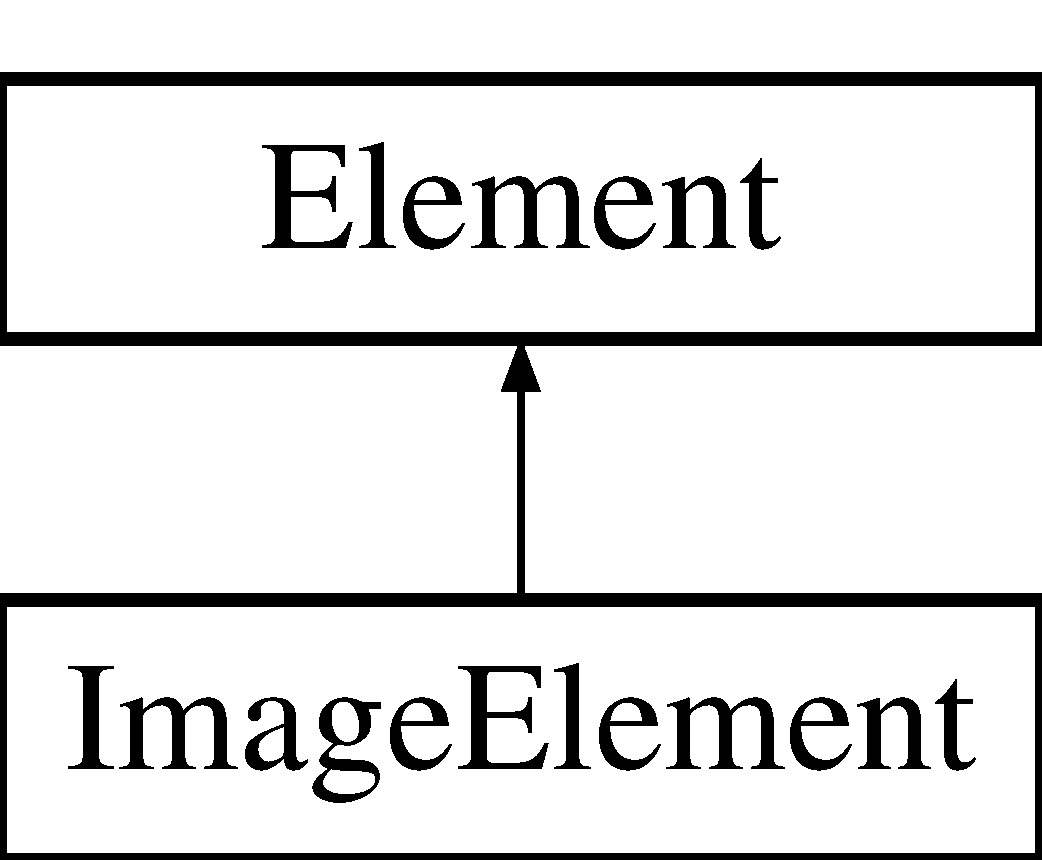
\includegraphics[height=2.000000cm]{class_image_element}
\end{center}
\end{figure}
\subsection*{Public Member Functions}
\begin{DoxyCompactItemize}
\item 
\hyperlink{class_image_element_a74aff4a808a295c0557f9c4dbedbc50a}{Image\-Element} ()
\item 
\hyperlink{class_image_element_aba9605d67c75b2802a45e93a4b0cff5d}{Image\-Element} (\hyperlink{class_image}{Image} \&img)
\item 
\hyperlink{class_image_element_a2a1f13235bc96229d3257212b3c62c79}{Image\-Element} (unsigned int x, unsigned int y)
\item 
\hyperlink{class_image_element_a9661aca27d32e6b9252dbbe45417f1bf}{Image\-Element} (unsigned int x, unsigned int y, unsigned int width, unsigned int height)
\item 
\hyperlink{class_image_element_a63993109c5c8e49f95c25ca13a887f1e}{Image\-Element} (unsigned int x, unsigned int y, unsigned int width, unsigned int height, \hyperlink{class_image}{Image} \&img)
\item 
void \hyperlink{class_image_element_aa785ef26786dc59b0e66a71e465b3e31}{clear\-Result} ()
\end{DoxyCompactItemize}
\subsection*{Additional Inherited Members}


\subsection{Detailed Description}


Definition at line 9 of file Image\-Element.\-h.



\subsection{Constructor \& Destructor Documentation}
\hypertarget{class_image_element_a74aff4a808a295c0557f9c4dbedbc50a}{\index{Image\-Element@{Image\-Element}!Image\-Element@{Image\-Element}}
\index{Image\-Element@{Image\-Element}!ImageElement@{Image\-Element}}
\subsubsection[{Image\-Element}]{\setlength{\rightskip}{0pt plus 5cm}Image\-Element\-::\-Image\-Element (
\begin{DoxyParamCaption}
{}
\end{DoxyParamCaption}
)\hspace{0.3cm}{\ttfamily [inline]}}}\label{class_image_element_a74aff4a808a295c0557f9c4dbedbc50a}


Definition at line 12 of file Image\-Element.\-h.

\hypertarget{class_image_element_aba9605d67c75b2802a45e93a4b0cff5d}{\index{Image\-Element@{Image\-Element}!Image\-Element@{Image\-Element}}
\index{Image\-Element@{Image\-Element}!ImageElement@{Image\-Element}}
\subsubsection[{Image\-Element}]{\setlength{\rightskip}{0pt plus 5cm}Image\-Element\-::\-Image\-Element (
\begin{DoxyParamCaption}
\item[{{\bf Image} \&}]{img}
\end{DoxyParamCaption}
)\hspace{0.3cm}{\ttfamily [inline]}}}\label{class_image_element_aba9605d67c75b2802a45e93a4b0cff5d}


Definition at line 13 of file Image\-Element.\-h.

\hypertarget{class_image_element_a2a1f13235bc96229d3257212b3c62c79}{\index{Image\-Element@{Image\-Element}!Image\-Element@{Image\-Element}}
\index{Image\-Element@{Image\-Element}!ImageElement@{Image\-Element}}
\subsubsection[{Image\-Element}]{\setlength{\rightskip}{0pt plus 5cm}Image\-Element\-::\-Image\-Element (
\begin{DoxyParamCaption}
\item[{unsigned int}]{x, }
\item[{unsigned int}]{y}
\end{DoxyParamCaption}
)\hspace{0.3cm}{\ttfamily [inline]}}}\label{class_image_element_a2a1f13235bc96229d3257212b3c62c79}


Definition at line 14 of file Image\-Element.\-h.

\hypertarget{class_image_element_a9661aca27d32e6b9252dbbe45417f1bf}{\index{Image\-Element@{Image\-Element}!Image\-Element@{Image\-Element}}
\index{Image\-Element@{Image\-Element}!ImageElement@{Image\-Element}}
\subsubsection[{Image\-Element}]{\setlength{\rightskip}{0pt plus 5cm}Image\-Element\-::\-Image\-Element (
\begin{DoxyParamCaption}
\item[{unsigned int}]{x, }
\item[{unsigned int}]{y, }
\item[{unsigned int}]{width, }
\item[{unsigned int}]{height}
\end{DoxyParamCaption}
)\hspace{0.3cm}{\ttfamily [inline]}}}\label{class_image_element_a9661aca27d32e6b9252dbbe45417f1bf}


Definition at line 17 of file Image\-Element.\-h.

\hypertarget{class_image_element_a63993109c5c8e49f95c25ca13a887f1e}{\index{Image\-Element@{Image\-Element}!Image\-Element@{Image\-Element}}
\index{Image\-Element@{Image\-Element}!ImageElement@{Image\-Element}}
\subsubsection[{Image\-Element}]{\setlength{\rightskip}{0pt plus 5cm}Image\-Element\-::\-Image\-Element (
\begin{DoxyParamCaption}
\item[{unsigned int}]{x, }
\item[{unsigned int}]{y, }
\item[{unsigned int}]{width, }
\item[{unsigned int}]{height, }
\item[{{\bf Image} \&}]{img}
\end{DoxyParamCaption}
)\hspace{0.3cm}{\ttfamily [inline]}}}\label{class_image_element_a63993109c5c8e49f95c25ca13a887f1e}


Definition at line 19 of file Image\-Element.\-h.



\subsection{Member Function Documentation}
\hypertarget{class_image_element_aa785ef26786dc59b0e66a71e465b3e31}{\index{Image\-Element@{Image\-Element}!clear\-Result@{clear\-Result}}
\index{clear\-Result@{clear\-Result}!ImageElement@{Image\-Element}}
\subsubsection[{clear\-Result}]{\setlength{\rightskip}{0pt plus 5cm}void Image\-Element\-::clear\-Result (
\begin{DoxyParamCaption}
{}
\end{DoxyParamCaption}
)\hspace{0.3cm}{\ttfamily [inline]}, {\ttfamily [virtual]}}}\label{class_image_element_aa785ef26786dc59b0e66a71e465b3e31}


Reimplemented from \hyperlink{class_element_a5a35a40d6797bf8b6ebe1b76090244fd}{Element}.



Definition at line 22 of file Image\-Element.\-h.



The documentation for this class was generated from the following file\-:\begin{DoxyCompactItemize}
\item 
image/\hyperlink{_image_element_8h}{Image\-Element.\-h}\end{DoxyCompactItemize}

\hypertarget{class_pixel}{\section{Pixel Class Reference}
\label{class_pixel}\index{Pixel@{Pixel}}
}


{\ttfamily \#include $<$Pixel.\-h$>$}

\subsection*{Public Member Functions}
\begin{DoxyCompactItemize}
\item 
\hyperlink{class_pixel_a27ad99a2f705e635c42d242d530d4756}{Pixel} ()
\item 
\hyperlink{class_pixel_a9ba4bf2d33c6d503e30059e61a43c045}{Pixel} (int R, int G, int B)
\item 
\hyperlink{class_pixel_a7a99c26ff5ea05251c24b5897443efda}{Pixel} (int R, int G, int B, int A)
\item 
\hyperlink{class_pixel_aa130b6db6edd3e7145a70a39c6eb2439}{Pixel} (\hyperlink{class_pixel}{Pixel} \&p)
\item 
void \hyperlink{class_pixel_a32492f5ea18dbc883b721948efe07764}{set\-R\-G\-B} (int R, int G, int B)
\item 
void \hyperlink{class_pixel_a58de4c2c1419fde30f4f3428eed66a0a}{set\-R\-G\-B\-A} (int R, int G, int B, int A)
\item 
int \hyperlink{class_pixel_afdb27eea61316a8f08cf10685e813dd5}{get\-R} () const 
\item 
int \hyperlink{class_pixel_ad1badd12caea7dba660ca7f5d0df241e}{get\-G} () const 
\item 
int \hyperlink{class_pixel_abce7ab2c36592c9ee041eb8ce68900b4}{get\-B} () const 
\item 
int \hyperlink{class_pixel_aea305b0ebe5f965236a6417edf83681d}{get\-A} () const 
\end{DoxyCompactItemize}
\subsection*{Friends}
\begin{DoxyCompactItemize}
\item 
std\-::ostream \& \hyperlink{class_pixel_a8162d24b145dcb53be8e5b1ba52df5be}{operator$<$$<$} (std\-::ostream \&out, const \hyperlink{class_pixel}{Pixel} \&p)
\end{DoxyCompactItemize}


\subsection{Detailed Description}


Definition at line 6 of file Pixel.\-h.



\subsection{Constructor \& Destructor Documentation}
\hypertarget{class_pixel_a27ad99a2f705e635c42d242d530d4756}{\index{Pixel@{Pixel}!Pixel@{Pixel}}
\index{Pixel@{Pixel}!Pixel@{Pixel}}
\subsubsection[{Pixel}]{\setlength{\rightskip}{0pt plus 5cm}Pixel\-::\-Pixel (
\begin{DoxyParamCaption}
{}
\end{DoxyParamCaption}
)}}\label{class_pixel_a27ad99a2f705e635c42d242d530d4756}


Definition at line 3 of file Pixel.\-cpp.

\hypertarget{class_pixel_a9ba4bf2d33c6d503e30059e61a43c045}{\index{Pixel@{Pixel}!Pixel@{Pixel}}
\index{Pixel@{Pixel}!Pixel@{Pixel}}
\subsubsection[{Pixel}]{\setlength{\rightskip}{0pt plus 5cm}Pixel\-::\-Pixel (
\begin{DoxyParamCaption}
\item[{int}]{R, }
\item[{int}]{G, }
\item[{int}]{B}
\end{DoxyParamCaption}
)}}\label{class_pixel_a9ba4bf2d33c6d503e30059e61a43c045}


Definition at line 4 of file Pixel.\-cpp.

\hypertarget{class_pixel_a7a99c26ff5ea05251c24b5897443efda}{\index{Pixel@{Pixel}!Pixel@{Pixel}}
\index{Pixel@{Pixel}!Pixel@{Pixel}}
\subsubsection[{Pixel}]{\setlength{\rightskip}{0pt plus 5cm}Pixel\-::\-Pixel (
\begin{DoxyParamCaption}
\item[{int}]{R, }
\item[{int}]{G, }
\item[{int}]{B, }
\item[{int}]{A}
\end{DoxyParamCaption}
)}}\label{class_pixel_a7a99c26ff5ea05251c24b5897443efda}


Definition at line 7 of file Pixel.\-cpp.

\hypertarget{class_pixel_aa130b6db6edd3e7145a70a39c6eb2439}{\index{Pixel@{Pixel}!Pixel@{Pixel}}
\index{Pixel@{Pixel}!Pixel@{Pixel}}
\subsubsection[{Pixel}]{\setlength{\rightskip}{0pt plus 5cm}Pixel\-::\-Pixel (
\begin{DoxyParamCaption}
\item[{{\bf Pixel} \&}]{p}
\end{DoxyParamCaption}
)}}\label{class_pixel_aa130b6db6edd3e7145a70a39c6eb2439}


Definition at line 11 of file Pixel.\-cpp.



\subsection{Member Function Documentation}
\hypertarget{class_pixel_aea305b0ebe5f965236a6417edf83681d}{\index{Pixel@{Pixel}!get\-A@{get\-A}}
\index{get\-A@{get\-A}!Pixel@{Pixel}}
\subsubsection[{get\-A}]{\setlength{\rightskip}{0pt plus 5cm}int Pixel\-::get\-A (
\begin{DoxyParamCaption}
{}
\end{DoxyParamCaption}
) const}}\label{class_pixel_aea305b0ebe5f965236a6417edf83681d}


Definition at line 34 of file Pixel.\-cpp.

\hypertarget{class_pixel_abce7ab2c36592c9ee041eb8ce68900b4}{\index{Pixel@{Pixel}!get\-B@{get\-B}}
\index{get\-B@{get\-B}!Pixel@{Pixel}}
\subsubsection[{get\-B}]{\setlength{\rightskip}{0pt plus 5cm}int Pixel\-::get\-B (
\begin{DoxyParamCaption}
{}
\end{DoxyParamCaption}
) const}}\label{class_pixel_abce7ab2c36592c9ee041eb8ce68900b4}


Definition at line 31 of file Pixel.\-cpp.

\hypertarget{class_pixel_ad1badd12caea7dba660ca7f5d0df241e}{\index{Pixel@{Pixel}!get\-G@{get\-G}}
\index{get\-G@{get\-G}!Pixel@{Pixel}}
\subsubsection[{get\-G}]{\setlength{\rightskip}{0pt plus 5cm}int Pixel\-::get\-G (
\begin{DoxyParamCaption}
{}
\end{DoxyParamCaption}
) const}}\label{class_pixel_ad1badd12caea7dba660ca7f5d0df241e}


Definition at line 28 of file Pixel.\-cpp.

\hypertarget{class_pixel_afdb27eea61316a8f08cf10685e813dd5}{\index{Pixel@{Pixel}!get\-R@{get\-R}}
\index{get\-R@{get\-R}!Pixel@{Pixel}}
\subsubsection[{get\-R}]{\setlength{\rightskip}{0pt plus 5cm}int Pixel\-::get\-R (
\begin{DoxyParamCaption}
{}
\end{DoxyParamCaption}
) const}}\label{class_pixel_afdb27eea61316a8f08cf10685e813dd5}


Definition at line 25 of file Pixel.\-cpp.

\hypertarget{class_pixel_a32492f5ea18dbc883b721948efe07764}{\index{Pixel@{Pixel}!set\-R\-G\-B@{set\-R\-G\-B}}
\index{set\-R\-G\-B@{set\-R\-G\-B}!Pixel@{Pixel}}
\subsubsection[{set\-R\-G\-B}]{\setlength{\rightskip}{0pt plus 5cm}void Pixel\-::set\-R\-G\-B (
\begin{DoxyParamCaption}
\item[{int}]{R, }
\item[{int}]{G, }
\item[{int}]{B}
\end{DoxyParamCaption}
)}}\label{class_pixel_a32492f5ea18dbc883b721948efe07764}


Definition at line 19 of file Pixel.\-cpp.

\hypertarget{class_pixel_a58de4c2c1419fde30f4f3428eed66a0a}{\index{Pixel@{Pixel}!set\-R\-G\-B\-A@{set\-R\-G\-B\-A}}
\index{set\-R\-G\-B\-A@{set\-R\-G\-B\-A}!Pixel@{Pixel}}
\subsubsection[{set\-R\-G\-B\-A}]{\setlength{\rightskip}{0pt plus 5cm}void Pixel\-::set\-R\-G\-B\-A (
\begin{DoxyParamCaption}
\item[{int}]{R, }
\item[{int}]{G, }
\item[{int}]{B, }
\item[{int}]{A}
\end{DoxyParamCaption}
)}}\label{class_pixel_a58de4c2c1419fde30f4f3428eed66a0a}


Definition at line 22 of file Pixel.\-cpp.



\subsection{Friends And Related Function Documentation}
\hypertarget{class_pixel_a8162d24b145dcb53be8e5b1ba52df5be}{\index{Pixel@{Pixel}!operator$<$$<$@{operator$<$$<$}}
\index{operator$<$$<$@{operator$<$$<$}!Pixel@{Pixel}}
\subsubsection[{operator$<$$<$}]{\setlength{\rightskip}{0pt plus 5cm}std\-::ostream\& operator$<$$<$ (
\begin{DoxyParamCaption}
\item[{std\-::ostream \&}]{out, }
\item[{const {\bf Pixel} \&}]{p}
\end{DoxyParamCaption}
)\hspace{0.3cm}{\ttfamily [friend]}}}\label{class_pixel_a8162d24b145dcb53be8e5b1ba52df5be}


Definition at line 37 of file Pixel.\-cpp.



The documentation for this class was generated from the following files\-:\begin{DoxyCompactItemize}
\item 
image/\hyperlink{_pixel_8h}{Pixel.\-h}\item 
image/\hyperlink{_pixel_8cpp}{Pixel.\-cpp}\end{DoxyCompactItemize}

\hypertarget{class_text}{\section{Text Class Reference}
\label{class_text}\index{Text@{Text}}
}


{\ttfamily \#include $<$Text.\-h$>$}

\subsection*{Public Member Functions}
\begin{DoxyCompactItemize}
\item 
\hyperlink{class_text_ab3e26143fccc52699bcc5149cae852bc}{Text} ()
\item 
\hyperlink{class_text_a961009f9b86e79ed9a325b5e2dd0f3ae}{Text} (\hyperlink{class_text}{Text} \&txt)
\item 
\hyperlink{class_text_a79ab4b6e0aeccad7c1afa0db4a476f38}{Text} (int w, int h, int size)
\item 
\hyperlink{class_text_a24e7df3620c8650eb81b825dbc9c3d1f}{Text} (int w, int h, int size, string c)
\item 
\hyperlink{class_text_a2d49e5c280e205125b149f7777ae30c7}{$\sim$\-Text} ()
\item 
void \hyperlink{class_text_a2004a4210f6a0b584bec7272b9cedcfb}{set\-Text} (string c)
\item 
\hyperlink{class_image}{Image} $\ast$ \hyperlink{class_text_ab70ee3b32a21afc611059d70f2b8d3e1}{get\-Image} ()
\item 
string \hyperlink{class_text_a3a51500bcaf5bd80c7d52975c5ba4e8e}{get\-Text} (void)
\end{DoxyCompactItemize}


\subsection{Detailed Description}


Definition at line 12 of file Text.\-h.



\subsection{Constructor \& Destructor Documentation}
\hypertarget{class_text_ab3e26143fccc52699bcc5149cae852bc}{\index{Text@{Text}!Text@{Text}}
\index{Text@{Text}!Text@{Text}}
\subsubsection[{Text}]{\setlength{\rightskip}{0pt plus 5cm}Text\-::\-Text (
\begin{DoxyParamCaption}
{}
\end{DoxyParamCaption}
)}}\label{class_text_ab3e26143fccc52699bcc5149cae852bc}


Definition at line 14 of file Text.\-cpp.

\hypertarget{class_text_a961009f9b86e79ed9a325b5e2dd0f3ae}{\index{Text@{Text}!Text@{Text}}
\index{Text@{Text}!Text@{Text}}
\subsubsection[{Text}]{\setlength{\rightskip}{0pt plus 5cm}Text\-::\-Text (
\begin{DoxyParamCaption}
\item[{{\bf Text} \&}]{txt}
\end{DoxyParamCaption}
)}}\label{class_text_a961009f9b86e79ed9a325b5e2dd0f3ae}


Definition at line 41 of file Text.\-cpp.

\hypertarget{class_text_a79ab4b6e0aeccad7c1afa0db4a476f38}{\index{Text@{Text}!Text@{Text}}
\index{Text@{Text}!Text@{Text}}
\subsubsection[{Text}]{\setlength{\rightskip}{0pt plus 5cm}Text\-::\-Text (
\begin{DoxyParamCaption}
\item[{int}]{w, }
\item[{int}]{h, }
\item[{int}]{size}
\end{DoxyParamCaption}
)}}\label{class_text_a79ab4b6e0aeccad7c1afa0db4a476f38}


Definition at line 19 of file Text.\-cpp.

\hypertarget{class_text_a24e7df3620c8650eb81b825dbc9c3d1f}{\index{Text@{Text}!Text@{Text}}
\index{Text@{Text}!Text@{Text}}
\subsubsection[{Text}]{\setlength{\rightskip}{0pt plus 5cm}Text\-::\-Text (
\begin{DoxyParamCaption}
\item[{int}]{w, }
\item[{int}]{h, }
\item[{int}]{size, }
\item[{string}]{c}
\end{DoxyParamCaption}
)}}\label{class_text_a24e7df3620c8650eb81b825dbc9c3d1f}


Definition at line 24 of file Text.\-cpp.

\hypertarget{class_text_a2d49e5c280e205125b149f7777ae30c7}{\index{Text@{Text}!$\sim$\-Text@{$\sim$\-Text}}
\index{$\sim$\-Text@{$\sim$\-Text}!Text@{Text}}
\subsubsection[{$\sim$\-Text}]{\setlength{\rightskip}{0pt plus 5cm}Text\-::$\sim$\-Text (
\begin{DoxyParamCaption}
{}
\end{DoxyParamCaption}
)}}\label{class_text_a2d49e5c280e205125b149f7777ae30c7}


Definition at line 46 of file Text.\-cpp.



\subsection{Member Function Documentation}
\hypertarget{class_text_ab70ee3b32a21afc611059d70f2b8d3e1}{\index{Text@{Text}!get\-Image@{get\-Image}}
\index{get\-Image@{get\-Image}!Text@{Text}}
\subsubsection[{get\-Image}]{\setlength{\rightskip}{0pt plus 5cm}{\bf Image} $\ast$ Text\-::get\-Image (
\begin{DoxyParamCaption}
{}
\end{DoxyParamCaption}
)}}\label{class_text_ab70ee3b32a21afc611059d70f2b8d3e1}


Definition at line 62 of file Text.\-cpp.

\hypertarget{class_text_a3a51500bcaf5bd80c7d52975c5ba4e8e}{\index{Text@{Text}!get\-Text@{get\-Text}}
\index{get\-Text@{get\-Text}!Text@{Text}}
\subsubsection[{get\-Text}]{\setlength{\rightskip}{0pt plus 5cm}string Text\-::get\-Text (
\begin{DoxyParamCaption}
\item[{void}]{}
\end{DoxyParamCaption}
)\hspace{0.3cm}{\ttfamily [inline]}}}\label{class_text_a3a51500bcaf5bd80c7d52975c5ba4e8e}


Definition at line 22 of file Text.\-h.

\hypertarget{class_text_a2004a4210f6a0b584bec7272b9cedcfb}{\index{Text@{Text}!set\-Text@{set\-Text}}
\index{set\-Text@{set\-Text}!Text@{Text}}
\subsubsection[{set\-Text}]{\setlength{\rightskip}{0pt plus 5cm}void Text\-::set\-Text (
\begin{DoxyParamCaption}
\item[{string}]{c}
\end{DoxyParamCaption}
)}}\label{class_text_a2004a4210f6a0b584bec7272b9cedcfb}


Definition at line 56 of file Text.\-cpp.



The documentation for this class was generated from the following files\-:\begin{DoxyCompactItemize}
\item 
text/\hyperlink{_text_8h}{Text.\-h}\item 
text/\hyperlink{_text_8cpp}{Text.\-cpp}\end{DoxyCompactItemize}

\hypertarget{class_text_element}{\section{Text\-Element Class Reference}
\label{class_text_element}\index{Text\-Element@{Text\-Element}}
}


The class used to store elements of text.  




{\ttfamily \#include $<$Text\-Element.\-h$>$}

Inheritance diagram for Text\-Element\-:\begin{figure}[H]
\begin{center}
\leavevmode
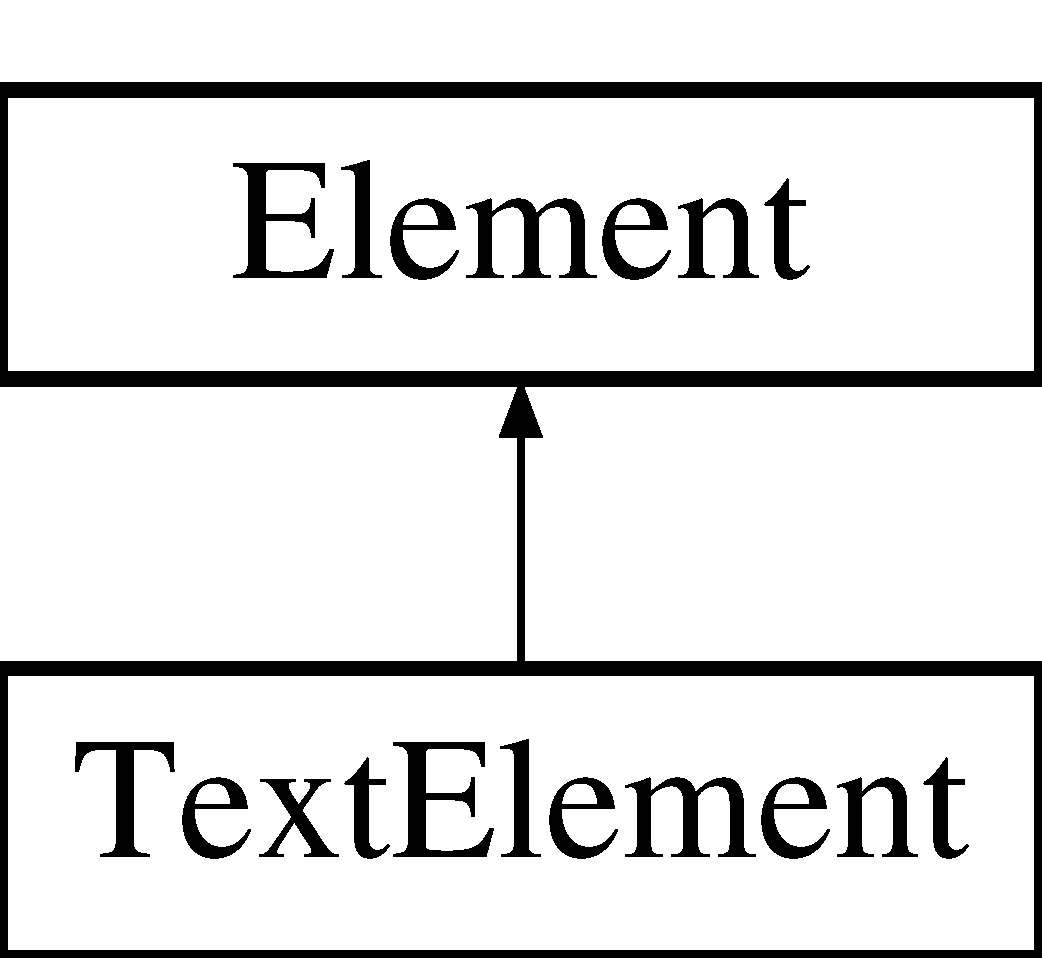
\includegraphics[height=2.000000cm]{class_text_element}
\end{center}
\end{figure}
\subsection*{Public Member Functions}
\begin{DoxyCompactItemize}
\item 
\hyperlink{class_text_element_aec15920e1f8e03bdd865ff3f6e0c396d}{Text\-Element} (unsigned int x, unsigned int y)
\begin{DoxyCompactList}\small\item\em Constructor. Sets x and y position of element. \end{DoxyCompactList}\item 
\hyperlink{class_text_element_ace1dec06df5c4a0635a4784b56a52b33}{Text\-Element} (unsigned int x, unsigned int y, unsigned int width, unsigned int height)
\begin{DoxyCompactList}\small\item\em Constructor. Sets x and y position of element along with height and width. \end{DoxyCompactList}\item 
\hyperlink{class_text_element_a288497cfc1863148bfc6ed9d8450f96b}{Text\-Element} (unsigned int x, unsigned int y, unsigned int width, unsigned int height, int size, string txt)
\begin{DoxyCompactList}\small\item\em Constructor. Sets x and y position of element along with height, width, font size and content. \end{DoxyCompactList}\item 
\hyperlink{class_text_element_a8638bd2628b9a0815bae74a8baf73c1f}{$\sim$\-Text\-Element} ()
\begin{DoxyCompactList}\small\item\em Destructor. \end{DoxyCompactList}\item 
void \hyperlink{class_text_element_a5f6f8013ecd934bd628ecaf6361bf03a}{set\-Text} (string txt)
\begin{DoxyCompactList}\small\item\em Updates the text stored and re-\/renders the result. \end{DoxyCompactList}\item 
void \hyperlink{class_text_element_a2d61f3953226d9d4d06d4003d6c33c34}{clear\-Result} ()
\begin{DoxyCompactList}\small\item\em Clears the rendered image previously stored. \end{DoxyCompactList}\end{DoxyCompactItemize}
\subsection*{Additional Inherited Members}


\subsection{Detailed Description}
The class used to store elements of text. 

Definition at line 13 of file Text\-Element.\-h.



\subsection{Constructor \& Destructor Documentation}
\hypertarget{class_text_element_aec15920e1f8e03bdd865ff3f6e0c396d}{\index{Text\-Element@{Text\-Element}!Text\-Element@{Text\-Element}}
\index{Text\-Element@{Text\-Element}!TextElement@{Text\-Element}}
\subsubsection[{Text\-Element}]{\setlength{\rightskip}{0pt plus 5cm}Text\-Element\-::\-Text\-Element (
\begin{DoxyParamCaption}
\item[{unsigned int}]{x, }
\item[{unsigned int}]{y}
\end{DoxyParamCaption}
)}}\label{class_text_element_aec15920e1f8e03bdd865ff3f6e0c396d}


Constructor. Sets x and y position of element. 

Constructor with just x,y position sets sizes to zero and font size to 1 and uses an empty string 

Definition at line 10 of file Text\-Element.\-cpp.

\hypertarget{class_text_element_ace1dec06df5c4a0635a4784b56a52b33}{\index{Text\-Element@{Text\-Element}!Text\-Element@{Text\-Element}}
\index{Text\-Element@{Text\-Element}!TextElement@{Text\-Element}}
\subsubsection[{Text\-Element}]{\setlength{\rightskip}{0pt plus 5cm}Text\-Element\-::\-Text\-Element (
\begin{DoxyParamCaption}
\item[{unsigned int}]{x, }
\item[{unsigned int}]{y, }
\item[{unsigned int}]{width, }
\item[{unsigned int}]{height}
\end{DoxyParamCaption}
)}}\label{class_text_element_ace1dec06df5c4a0635a4784b56a52b33}


Constructor. Sets x and y position of element along with height and width. 

Constructor with x,y position, width and height sets font size to 1 and an empty string 

Definition at line 15 of file Text\-Element.\-cpp.

\hypertarget{class_text_element_a288497cfc1863148bfc6ed9d8450f96b}{\index{Text\-Element@{Text\-Element}!Text\-Element@{Text\-Element}}
\index{Text\-Element@{Text\-Element}!TextElement@{Text\-Element}}
\subsubsection[{Text\-Element}]{\setlength{\rightskip}{0pt plus 5cm}Text\-Element\-::\-Text\-Element (
\begin{DoxyParamCaption}
\item[{unsigned int}]{x, }
\item[{unsigned int}]{y, }
\item[{unsigned int}]{width, }
\item[{unsigned int}]{height, }
\item[{int}]{size, }
\item[{string}]{txt}
\end{DoxyParamCaption}
)}}\label{class_text_element_a288497cfc1863148bfc6ed9d8450f96b}


Constructor. Sets x and y position of element along with height, width, font size and content. 

Constructor sets all variables and dynamically creates a \hyperlink{class_text}{Text} object 

Definition at line 20 of file Text\-Element.\-cpp.

\hypertarget{class_text_element_a8638bd2628b9a0815bae74a8baf73c1f}{\index{Text\-Element@{Text\-Element}!$\sim$\-Text\-Element@{$\sim$\-Text\-Element}}
\index{$\sim$\-Text\-Element@{$\sim$\-Text\-Element}!TextElement@{Text\-Element}}
\subsubsection[{$\sim$\-Text\-Element}]{\setlength{\rightskip}{0pt plus 5cm}Text\-Element\-::$\sim$\-Text\-Element (
\begin{DoxyParamCaption}
{}
\end{DoxyParamCaption}
)}}\label{class_text_element_a8638bd2628b9a0815bae74a8baf73c1f}


Destructor. 

Destructor deletes dynamically allocated variables if needed 

Definition at line 27 of file Text\-Element.\-cpp.



\subsection{Member Function Documentation}
\hypertarget{class_text_element_a2d61f3953226d9d4d06d4003d6c33c34}{\index{Text\-Element@{Text\-Element}!clear\-Result@{clear\-Result}}
\index{clear\-Result@{clear\-Result}!TextElement@{Text\-Element}}
\subsubsection[{clear\-Result}]{\setlength{\rightskip}{0pt plus 5cm}void Text\-Element\-::clear\-Result (
\begin{DoxyParamCaption}
{}
\end{DoxyParamCaption}
)\hspace{0.3cm}{\ttfamily [virtual]}}}\label{class_text_element_a2d61f3953226d9d4d06d4003d6c33c34}


Clears the rendered image previously stored. 

Clears the rendered image we have stored 

Reimplemented from \hyperlink{class_element_a7a110bce4630cd7b35b1c2d401774598}{Element}.



Definition at line 39 of file Text\-Element.\-cpp.

\hypertarget{class_text_element_a5f6f8013ecd934bd628ecaf6361bf03a}{\index{Text\-Element@{Text\-Element}!set\-Text@{set\-Text}}
\index{set\-Text@{set\-Text}!TextElement@{Text\-Element}}
\subsubsection[{set\-Text}]{\setlength{\rightskip}{0pt plus 5cm}void Text\-Element\-::set\-Text (
\begin{DoxyParamCaption}
\item[{string}]{txt}
\end{DoxyParamCaption}
)}}\label{class_text_element_a5f6f8013ecd934bd628ecaf6361bf03a}


Updates the text stored and re-\/renders the result. 

Updates the value of the text which renders the text 

Definition at line 34 of file Text\-Element.\-cpp.



The documentation for this class was generated from the following files\-:\begin{DoxyCompactItemize}
\item 
text/\hyperlink{_text_element_8h}{Text\-Element.\-h}\item 
text/\hyperlink{_text_element_8cpp}{Text\-Element.\-cpp}\end{DoxyCompactItemize}

\hypertarget{class_toggle_button}{\section{Toggle\-Button Class Reference}
\label{class_toggle_button}\index{Toggle\-Button@{Toggle\-Button}}
}


{\ttfamily \#include $<$Toggle\-Button.\-h$>$}

Inheritance diagram for Toggle\-Button\-:\begin{figure}[H]
\begin{center}
\leavevmode
\includegraphics[height=3.000000cm]{class_toggle_button}
\end{center}
\end{figure}
\subsection*{Public Member Functions}
\begin{DoxyCompactItemize}
\item 
\hyperlink{class_toggle_button_aa978ecd118f11987b5a8060072b407f0}{Toggle\-Button} ()
\item 
\hyperlink{class_toggle_button_aef2a0abd79b023f9a4bcb5b53fc5be59}{Toggle\-Button} (int x, int y)
\item 
\hyperlink{class_toggle_button_a1217ac37ca79450eeaf8a8a7cd79e690}{Toggle\-Button} (int x, int y, int w, int h)
\item 
\hyperlink{class_toggle_button_a7ae1419f6fe7bc72af6e972c490f3d3c}{Toggle\-Button} (int x, int y, int w, int h, string txt)
\item 
\hyperlink{class_toggle_button_adf501f89389fb0297e5b1b9ceaf1abdc}{Toggle\-Button} (int x, int y, int w, int h, string content, int size, \hyperlink{class_image_element}{Image\-Element} $\ast$i)
\end{DoxyCompactItemize}
\subsection*{Additional Inherited Members}


\subsection{Detailed Description}


Definition at line 12 of file Toggle\-Button.\-h.



\subsection{Constructor \& Destructor Documentation}
\hypertarget{class_toggle_button_aa978ecd118f11987b5a8060072b407f0}{\index{Toggle\-Button@{Toggle\-Button}!Toggle\-Button@{Toggle\-Button}}
\index{Toggle\-Button@{Toggle\-Button}!ToggleButton@{Toggle\-Button}}
\subsubsection[{Toggle\-Button}]{\setlength{\rightskip}{0pt plus 5cm}Toggle\-Button\-::\-Toggle\-Button (
\begin{DoxyParamCaption}
{}
\end{DoxyParamCaption}
)\hspace{0.3cm}{\ttfamily [inline]}}}\label{class_toggle_button_aa978ecd118f11987b5a8060072b407f0}


Definition at line 14 of file Toggle\-Button.\-h.

\hypertarget{class_toggle_button_aef2a0abd79b023f9a4bcb5b53fc5be59}{\index{Toggle\-Button@{Toggle\-Button}!Toggle\-Button@{Toggle\-Button}}
\index{Toggle\-Button@{Toggle\-Button}!ToggleButton@{Toggle\-Button}}
\subsubsection[{Toggle\-Button}]{\setlength{\rightskip}{0pt plus 5cm}Toggle\-Button\-::\-Toggle\-Button (
\begin{DoxyParamCaption}
\item[{int}]{x, }
\item[{int}]{y}
\end{DoxyParamCaption}
)\hspace{0.3cm}{\ttfamily [inline]}}}\label{class_toggle_button_aef2a0abd79b023f9a4bcb5b53fc5be59}


Definition at line 15 of file Toggle\-Button.\-h.

\hypertarget{class_toggle_button_a1217ac37ca79450eeaf8a8a7cd79e690}{\index{Toggle\-Button@{Toggle\-Button}!Toggle\-Button@{Toggle\-Button}}
\index{Toggle\-Button@{Toggle\-Button}!ToggleButton@{Toggle\-Button}}
\subsubsection[{Toggle\-Button}]{\setlength{\rightskip}{0pt plus 5cm}Toggle\-Button\-::\-Toggle\-Button (
\begin{DoxyParamCaption}
\item[{int}]{x, }
\item[{int}]{y, }
\item[{int}]{w, }
\item[{int}]{h}
\end{DoxyParamCaption}
)\hspace{0.3cm}{\ttfamily [inline]}}}\label{class_toggle_button_a1217ac37ca79450eeaf8a8a7cd79e690}


Definition at line 16 of file Toggle\-Button.\-h.

\hypertarget{class_toggle_button_a7ae1419f6fe7bc72af6e972c490f3d3c}{\index{Toggle\-Button@{Toggle\-Button}!Toggle\-Button@{Toggle\-Button}}
\index{Toggle\-Button@{Toggle\-Button}!ToggleButton@{Toggle\-Button}}
\subsubsection[{Toggle\-Button}]{\setlength{\rightskip}{0pt plus 5cm}Toggle\-Button\-::\-Toggle\-Button (
\begin{DoxyParamCaption}
\item[{int}]{x, }
\item[{int}]{y, }
\item[{int}]{w, }
\item[{int}]{h, }
\item[{string}]{txt}
\end{DoxyParamCaption}
)\hspace{0.3cm}{\ttfamily [inline]}}}\label{class_toggle_button_a7ae1419f6fe7bc72af6e972c490f3d3c}


Definition at line 19 of file Toggle\-Button.\-h.

\hypertarget{class_toggle_button_adf501f89389fb0297e5b1b9ceaf1abdc}{\index{Toggle\-Button@{Toggle\-Button}!Toggle\-Button@{Toggle\-Button}}
\index{Toggle\-Button@{Toggle\-Button}!ToggleButton@{Toggle\-Button}}
\subsubsection[{Toggle\-Button}]{\setlength{\rightskip}{0pt plus 5cm}Toggle\-Button\-::\-Toggle\-Button (
\begin{DoxyParamCaption}
\item[{int}]{x, }
\item[{int}]{y, }
\item[{int}]{w, }
\item[{int}]{h, }
\item[{string}]{content, }
\item[{int}]{size, }
\item[{{\bf Image\-Element} $\ast$}]{i}
\end{DoxyParamCaption}
)\hspace{0.3cm}{\ttfamily [inline]}}}\label{class_toggle_button_adf501f89389fb0297e5b1b9ceaf1abdc}


Definition at line 23 of file Toggle\-Button.\-h.



The documentation for this class was generated from the following file\-:\begin{DoxyCompactItemize}
\item 
togglebutton/\hyperlink{_toggle_button_8h}{Toggle\-Button.\-h}\end{DoxyCompactItemize}

\chapter{File Documentation}
\hypertarget{_button_8h}{\section{button/\-Button.h File Reference}
\label{_button_8h}\index{button/\-Button.\-h@{button/\-Button.\-h}}
}
{\ttfamily \#include $<$string$>$}\\*
{\ttfamily \#include \char`\"{}../image/\-Image.\-h\char`\"{}}\\*
{\ttfamily \#include \char`\"{}../text/\-Text.\-h\char`\"{}}\\*
{\ttfamily \#include \char`\"{}../element/\-Element.\-h\char`\"{}}\\*
{\ttfamily \#include \char`\"{}../image/\-Image\-Element.\-h\char`\"{}}\\*
{\ttfamily \#include \char`\"{}../text/\-Text\-Element.\-h\char`\"{}}\\*
\subsection*{Classes}
\begin{DoxyCompactItemize}
\item 
class \hyperlink{class_button}{Button}
\begin{DoxyCompactList}\small\item\em The class used to store buttons consisting of a background image and a foreground text. \end{DoxyCompactList}\end{DoxyCompactItemize}


\subsection{Detailed Description}
This file contains the \hyperlink{class_button}{Button} class. 

Definition in file \hyperlink{_button_8h_source}{Button.\-h}.


\hypertarget{button_2main_8cpp}{\section{button/main.cpp File Reference}
\label{button_2main_8cpp}\index{button/main.\-cpp@{button/main.\-cpp}}
}
{\ttfamily \#include $<$string$>$}\\*
{\ttfamily \#include \char`\"{}../image/\-Image.\-h\char`\"{}}\\*
{\ttfamily \#include \char`\"{}../image/\-Pixel.\-h\char`\"{}}\\*
{\ttfamily \#include \char`\"{}../text/\-Text.\-h\char`\"{}}\\*
{\ttfamily \#include \char`\"{}Button.\-h\char`\"{}}\\*
\subsection*{Functions}
\begin{DoxyCompactItemize}
\item 
int \hyperlink{button_2main_8cpp_ae66f6b31b5ad750f1fe042a706a4e3d4}{main} ()
\end{DoxyCompactItemize}


\subsection{Function Documentation}
\hypertarget{button_2main_8cpp_ae66f6b31b5ad750f1fe042a706a4e3d4}{\index{button/main.\-cpp@{button/main.\-cpp}!main@{main}}
\index{main@{main}!button/main.cpp@{button/main.\-cpp}}
\subsubsection[{main}]{\setlength{\rightskip}{0pt plus 5cm}int main (
\begin{DoxyParamCaption}
{}
\end{DoxyParamCaption}
)}}\label{button_2main_8cpp_ae66f6b31b5ad750f1fe042a706a4e3d4}


Definition at line 9 of file main.\-cpp.


\hypertarget{main_8cpp}{\section{main.\-cpp File Reference}
\label{main_8cpp}\index{main.\-cpp@{main.\-cpp}}
}
{\ttfamily \#include $<$G\-L/glfw.\-h$>$}\\*
{\ttfamily \#include $<$Free\-Image.\-h$>$}\\*
{\ttfamily \#include $<$stdlib.\-h$>$}\\*
{\ttfamily \#include $<$stdio.\-h$>$}\\*
{\ttfamily \#include $<$iostream$>$}\\*
{\ttfamily \#include \char`\"{}main.\-h\char`\"{}}\\*
{\ttfamily \#include \char`\"{}element/\-Element.\-h\char`\"{}}\\*
{\ttfamily \#include \char`\"{}text/\-Text\-Element.\-h\char`\"{}}\\*
{\ttfamily \#include \char`\"{}image/\-Image\-Element.\-h\char`\"{}}\\*
{\ttfamily \#include \char`\"{}togglebutton/\-Toggle\-Button.\-h\char`\"{}}\\*
{\ttfamily \#include \char`\"{}button/\-Button.\-h\char`\"{}}\\*
\subsection*{Functions}
\begin{DoxyCompactItemize}
\item 
int \hyperlink{main_8cpp_ae66f6b31b5ad750f1fe042a706a4e3d4}{main} ()
\item 
int \hyperlink{main_8cpp_ad081815fa97a33e7833e875910f03c74}{load\-Gui\-Texture} (string texture\-String)
\item 
void \hyperlink{main_8cpp_a2a026e829d973a118ea722a2296d564a}{shut\-Down} (int return\-Code)
\item 
int \hyperlink{main_8cpp_a078eadbd02baa0e3e49c38e8144eab3e}{close\-Window} (void)
\item 
void \hyperlink{main_8cpp_a2858154e2009b0e6e616f313177762bc}{init} (void)
\item 
void \hyperlink{main_8cpp_a52387bf053883d1a8feeee2dd2cdd4f3}{main\-Loop} (void)
\item 
void \hyperlink{main_8cpp_ad2e97e7b54d0bf35e406b91fbdd2f256}{draw} (void)
\item 
void G\-L\-F\-W\-C\-A\-L\-L \hyperlink{main_8cpp_a95681cbe7df715737b55654aa59ad866}{window\-Resize} (int width, int height)
\item 
void G\-L\-F\-W\-C\-A\-L\-L \hyperlink{main_8cpp_ae3cb3094e9a69387d1aaeac1c2189812}{mouse\-Clicked} (int m\-Button, int clicked)
\item 
void \hyperlink{main_8cpp_aded8f05225ff190aa74403c62a52020e}{button\-Clicked} (void $\ast$e)
\end{DoxyCompactItemize}
\subsection*{Variables}
\begin{DoxyCompactItemize}
\item 
G\-Luint \hyperlink{main_8cpp_a0704dfe56dec926cb35f7bdc0834ecd0}{texture}
\end{DoxyCompactItemize}


\subsection{Function Documentation}
\hypertarget{main_8cpp_aded8f05225ff190aa74403c62a52020e}{\index{main.\-cpp@{main.\-cpp}!button\-Clicked@{button\-Clicked}}
\index{button\-Clicked@{button\-Clicked}!main.cpp@{main.\-cpp}}
\subsubsection[{button\-Clicked}]{\setlength{\rightskip}{0pt plus 5cm}void button\-Clicked (
\begin{DoxyParamCaption}
\item[{void $\ast$}]{e}
\end{DoxyParamCaption}
)}}\label{main_8cpp_aded8f05225ff190aa74403c62a52020e}


Definition at line 209 of file main.\-cpp.

\hypertarget{main_8cpp_a078eadbd02baa0e3e49c38e8144eab3e}{\index{main.\-cpp@{main.\-cpp}!close\-Window@{close\-Window}}
\index{close\-Window@{close\-Window}!main.cpp@{main.\-cpp}}
\subsubsection[{close\-Window}]{\setlength{\rightskip}{0pt plus 5cm}int close\-Window (
\begin{DoxyParamCaption}
\item[{void}]{}
\end{DoxyParamCaption}
)}}\label{main_8cpp_a078eadbd02baa0e3e49c38e8144eab3e}


Definition at line 110 of file main.\-cpp.

\hypertarget{main_8cpp_ad2e97e7b54d0bf35e406b91fbdd2f256}{\index{main.\-cpp@{main.\-cpp}!draw@{draw}}
\index{draw@{draw}!main.cpp@{main.\-cpp}}
\subsubsection[{draw}]{\setlength{\rightskip}{0pt plus 5cm}void draw (
\begin{DoxyParamCaption}
\item[{void}]{}
\end{DoxyParamCaption}
)}}\label{main_8cpp_ad2e97e7b54d0bf35e406b91fbdd2f256}


Definition at line 169 of file main.\-cpp.

\hypertarget{main_8cpp_a2858154e2009b0e6e616f313177762bc}{\index{main.\-cpp@{main.\-cpp}!init@{init}}
\index{init@{init}!main.cpp@{main.\-cpp}}
\subsubsection[{init}]{\setlength{\rightskip}{0pt plus 5cm}void init (
\begin{DoxyParamCaption}
\item[{void}]{}
\end{DoxyParamCaption}
)}}\label{main_8cpp_a2858154e2009b0e6e616f313177762bc}
Initializes a glfw window for use in the demo

Definition at line 115 of file main.\-cpp.

\hypertarget{main_8cpp_ad081815fa97a33e7833e875910f03c74}{\index{main.\-cpp@{main.\-cpp}!load\-Gui\-Texture@{load\-Gui\-Texture}}
\index{load\-Gui\-Texture@{load\-Gui\-Texture}!main.cpp@{main.\-cpp}}
\subsubsection[{load\-Gui\-Texture}]{\setlength{\rightskip}{0pt plus 5cm}int load\-Gui\-Texture (
\begin{DoxyParamCaption}
\item[{string}]{texture\-String}
\end{DoxyParamCaption}
)}}\label{main_8cpp_ad081815fa97a33e7833e875910f03c74}


Definition at line 30 of file main.\-cpp.

\hypertarget{main_8cpp_ae66f6b31b5ad750f1fe042a706a4e3d4}{\index{main.\-cpp@{main.\-cpp}!main@{main}}
\index{main@{main}!main.cpp@{main.\-cpp}}
\subsubsection[{main}]{\setlength{\rightskip}{0pt plus 5cm}int main (
\begin{DoxyParamCaption}
{}
\end{DoxyParamCaption}
)}}\label{main_8cpp_ae66f6b31b5ad750f1fe042a706a4e3d4}


Definition at line 23 of file main.\-cpp.

\hypertarget{main_8cpp_a52387bf053883d1a8feeee2dd2cdd4f3}{\index{main.\-cpp@{main.\-cpp}!main\-Loop@{main\-Loop}}
\index{main\-Loop@{main\-Loop}!main.cpp@{main.\-cpp}}
\subsubsection[{main\-Loop}]{\setlength{\rightskip}{0pt plus 5cm}void main\-Loop (
\begin{DoxyParamCaption}
\item[{void}]{}
\end{DoxyParamCaption}
)}}\label{main_8cpp_a52387bf053883d1a8feeee2dd2cdd4f3}
the main event loop for the demo

Definition at line 153 of file main.\-cpp.

\hypertarget{main_8cpp_ae3cb3094e9a69387d1aaeac1c2189812}{\index{main.\-cpp@{main.\-cpp}!mouse\-Clicked@{mouse\-Clicked}}
\index{mouse\-Clicked@{mouse\-Clicked}!main.cpp@{main.\-cpp}}
\subsubsection[{mouse\-Clicked}]{\setlength{\rightskip}{0pt plus 5cm}void G\-L\-F\-W\-C\-A\-L\-L mouse\-Clicked (
\begin{DoxyParamCaption}
\item[{int}]{m\-Button, }
\item[{int}]{clicked}
\end{DoxyParamCaption}
)}}\label{main_8cpp_ae3cb3094e9a69387d1aaeac1c2189812}


Definition at line 198 of file main.\-cpp.

\hypertarget{main_8cpp_a2a026e829d973a118ea722a2296d564a}{\index{main.\-cpp@{main.\-cpp}!shut\-Down@{shut\-Down}}
\index{shut\-Down@{shut\-Down}!main.cpp@{main.\-cpp}}
\subsubsection[{shut\-Down}]{\setlength{\rightskip}{0pt plus 5cm}void shut\-Down (
\begin{DoxyParamCaption}
\item[{int}]{return\-Code}
\end{DoxyParamCaption}
)}}\label{main_8cpp_a2a026e829d973a118ea722a2296d564a}
shuts down glfw and exits the program with a return code

Definition at line 101 of file main.\-cpp.

\hypertarget{main_8cpp_a95681cbe7df715737b55654aa59ad866}{\index{main.\-cpp@{main.\-cpp}!window\-Resize@{window\-Resize}}
\index{window\-Resize@{window\-Resize}!main.cpp@{main.\-cpp}}
\subsubsection[{window\-Resize}]{\setlength{\rightskip}{0pt plus 5cm}void G\-L\-F\-W\-C\-A\-L\-L window\-Resize (
\begin{DoxyParamCaption}
\item[{int}]{width, }
\item[{int}]{height}
\end{DoxyParamCaption}
)}}\label{main_8cpp_a95681cbe7df715737b55654aa59ad866}


Definition at line 193 of file main.\-cpp.



\subsection{Variable Documentation}
\hypertarget{main_8cpp_a0704dfe56dec926cb35f7bdc0834ecd0}{\index{main.\-cpp@{main.\-cpp}!texture@{texture}}
\index{texture@{texture}!main.cpp@{main.\-cpp}}
\subsubsection[{texture}]{\setlength{\rightskip}{0pt plus 5cm}G\-Luint texture}}\label{main_8cpp_a0704dfe56dec926cb35f7bdc0834ecd0}


Definition at line 19 of file main.\-cpp.


\hypertarget{text_2main_8cpp}{\section{text/main.cpp File Reference}
\label{text_2main_8cpp}\index{text/main.\-cpp@{text/main.\-cpp}}
}
{\ttfamily \#include $<$iostream$>$}\\*
{\ttfamily \#include $<$string$>$}\\*
{\ttfamily \#include \char`\"{}Text.\-h\char`\"{}}\\*
{\ttfamily \#include \char`\"{}../image/\-Image.\-h\char`\"{}}\\*
\subsection*{Functions}
\begin{DoxyCompactItemize}
\item 
int \hyperlink{text_2main_8cpp_ae66f6b31b5ad750f1fe042a706a4e3d4}{main} ()
\end{DoxyCompactItemize}


\subsection{Function Documentation}
\hypertarget{text_2main_8cpp_ae66f6b31b5ad750f1fe042a706a4e3d4}{\index{text/main.\-cpp@{text/main.\-cpp}!main@{main}}
\index{main@{main}!text/main.cpp@{text/main.\-cpp}}
\subsubsection[{main}]{\setlength{\rightskip}{0pt plus 5cm}int main (
\begin{DoxyParamCaption}
{}
\end{DoxyParamCaption}
)}}\label{text_2main_8cpp_ae66f6b31b5ad750f1fe042a706a4e3d4}


Definition at line 7 of file main.\-cpp.


\hypertarget{_check_box_8h}{\section{checkbox/\-Check\-Box.h File Reference}
\label{_check_box_8h}\index{checkbox/\-Check\-Box.\-h@{checkbox/\-Check\-Box.\-h}}
}
{\ttfamily \#include \char`\"{}Element.\-h\char`\"{}}\\*
{\ttfamily \#include \char`\"{}Text.\-h\char`\"{}}\\*
{\ttfamily \#include \char`\"{}Image.\-h\char`\"{}}\\*
{\ttfamily \#include \char`\"{}Image\-Element.\-h\char`\"{}}\\*
{\ttfamily \#include \char`\"{}Text\-Element.\-h\char`\"{}}\\*
\subsection*{Classes}
\begin{DoxyCompactItemize}
\item 
class \hyperlink{class_check_box}{Check\-Box}
\end{DoxyCompactItemize}

\hypertarget{_element_8cpp}{\section{element/\-Element.cpp File Reference}
\label{_element_8cpp}\index{element/\-Element.\-cpp@{element/\-Element.\-cpp}}
}
{\ttfamily \#include \char`\"{}Element.\-h\char`\"{}}\\*
{\ttfamily \#include $<$iostream$>$}\\*
{\ttfamily \#include $<$algorithm$>$}\\*
{\ttfamily \#include $<$stdio.\-h$>$}\\*
{\ttfamily \#include \char`\"{}../image/\-Image.\-h\char`\"{}}\\*

\hypertarget{_element_8h}{\section{Element.\-h File Reference}
\label{_element_8h}\index{Element.\-h@{Element.\-h}}
}
{\ttfamily \#include $<$vector$>$}\\*
{\ttfamily \#include $<$algorithm$>$}\\*
{\ttfamily \#include \char`\"{}../image/\-Image.\-h\char`\"{}}\\*
\subsection*{Classes}
\begin{DoxyCompactItemize}
\item 
class \hyperlink{class_element}{Element}
\begin{DoxyCompactList}\small\item\em The base class that all G\-U\-I elements derive from. \end{DoxyCompactList}\end{DoxyCompactItemize}


\subsection{Detailed Description}
This file contains the \hyperlink{class_element}{Element} class. 

Definition in file \hyperlink{_element_8h_source}{Element.\-h}.


\input{element_2_main_8cpp}
\hypertarget{image_2_main_8cpp}{\section{image/\-Main.cpp File Reference}
\label{image_2_main_8cpp}\index{image/\-Main.\-cpp@{image/\-Main.\-cpp}}
}
{\ttfamily \#include $<$iostream$>$}\\*
{\ttfamily \#include \char`\"{}Image.\-h\char`\"{}}\\*
\subsection*{Functions}
\begin{DoxyCompactItemize}
\item 
int \hyperlink{image_2_main_8cpp_ae66f6b31b5ad750f1fe042a706a4e3d4}{main} ()
\end{DoxyCompactItemize}


\subsection{Function Documentation}
\hypertarget{image_2_main_8cpp_ae66f6b31b5ad750f1fe042a706a4e3d4}{\index{image/\-Main.\-cpp@{image/\-Main.\-cpp}!main@{main}}
\index{main@{main}!image/Main.cpp@{image/\-Main.\-cpp}}
\subsubsection[{main}]{\setlength{\rightskip}{0pt plus 5cm}int main (
\begin{DoxyParamCaption}
{}
\end{DoxyParamCaption}
)}}\label{image_2_main_8cpp_ae66f6b31b5ad750f1fe042a706a4e3d4}


Definition at line 5 of file Main.\-cpp.


\hypertarget{togglebutton_2_main_8cpp}{\section{togglebutton/\-Main.cpp File Reference}
\label{togglebutton_2_main_8cpp}\index{togglebutton/\-Main.\-cpp@{togglebutton/\-Main.\-cpp}}
}
{\ttfamily \#include $<$string$>$}\\*
{\ttfamily \#include \char`\"{}../image/\-Image.\-h\char`\"{}}\\*
{\ttfamily \#include \char`\"{}../image/\-Pixel.\-h\char`\"{}}\\*
{\ttfamily \#include \char`\"{}../text/\-Text.\-h\char`\"{}}\\*
{\ttfamily \#include \char`\"{}Button.\-h\char`\"{}}\\*
\subsection*{Functions}
\begin{DoxyCompactItemize}
\item 
int \hyperlink{togglebutton_2_main_8cpp_ae66f6b31b5ad750f1fe042a706a4e3d4}{main} ()
\end{DoxyCompactItemize}


\subsection{Function Documentation}
\hypertarget{togglebutton_2_main_8cpp_ae66f6b31b5ad750f1fe042a706a4e3d4}{\index{togglebutton/\-Main.\-cpp@{togglebutton/\-Main.\-cpp}!main@{main}}
\index{main@{main}!togglebutton/Main.cpp@{togglebutton/\-Main.\-cpp}}
\subsubsection[{main}]{\setlength{\rightskip}{0pt plus 5cm}int main (
\begin{DoxyParamCaption}
{}
\end{DoxyParamCaption}
)}}\label{togglebutton_2_main_8cpp_ae66f6b31b5ad750f1fe042a706a4e3d4}


Definition at line 9 of file Main.\-cpp.


\hypertarget{_image_8cpp}{\section{image/\-Image.cpp File Reference}
\label{_image_8cpp}\index{image/\-Image.\-cpp@{image/\-Image.\-cpp}}
}
{\ttfamily \#include \char`\"{}Image.\-h\char`\"{}}\\*
{\ttfamily \#include $<$algorithm$>$}\\*
\subsection*{Functions}
\begin{DoxyCompactItemize}
\item 
std\-::ostream \& \hyperlink{_image_8cpp_a7f50d34e230853ed6c2e8e288d543fc7}{operator$<$$<$} (std\-::ostream \&out, const \hyperlink{class_image}{Image} \&img)
\end{DoxyCompactItemize}
\subsection*{Variables}
\begin{DoxyCompactItemize}
\item 
\hyperlink{class_pixel}{Pixel} \hyperlink{_image_8cpp_a957a99086d859cea385db4395d24019e}{E\-R\-R\-O\-R\-P\-I\-X\-E\-L}
\end{DoxyCompactItemize}


\subsection{Function Documentation}
\hypertarget{_image_8cpp_a7f50d34e230853ed6c2e8e288d543fc7}{\index{Image.\-cpp@{Image.\-cpp}!operator$<$$<$@{operator$<$$<$}}
\index{operator$<$$<$@{operator$<$$<$}!Image.cpp@{Image.\-cpp}}
\subsubsection[{operator$<$$<$}]{\setlength{\rightskip}{0pt plus 5cm}std\-::ostream\& operator$<$$<$ (
\begin{DoxyParamCaption}
\item[{std\-::ostream \&}]{out, }
\item[{const {\bf Image} \&}]{img}
\end{DoxyParamCaption}
)}}\label{_image_8cpp_a7f50d34e230853ed6c2e8e288d543fc7}


Definition at line 147 of file Image.\-cpp.



\subsection{Variable Documentation}
\hypertarget{_image_8cpp_a957a99086d859cea385db4395d24019e}{\index{Image.\-cpp@{Image.\-cpp}!E\-R\-R\-O\-R\-P\-I\-X\-E\-L@{E\-R\-R\-O\-R\-P\-I\-X\-E\-L}}
\index{E\-R\-R\-O\-R\-P\-I\-X\-E\-L@{E\-R\-R\-O\-R\-P\-I\-X\-E\-L}!Image.cpp@{Image.\-cpp}}
\subsubsection[{E\-R\-R\-O\-R\-P\-I\-X\-E\-L}]{\setlength{\rightskip}{0pt plus 5cm}{\bf Pixel} E\-R\-R\-O\-R\-P\-I\-X\-E\-L}}\label{_image_8cpp_a957a99086d859cea385db4395d24019e}


Definition at line 101 of file Image.\-cpp.


\hypertarget{_image_8h}{\section{image/\-Image.h File Reference}
\label{_image_8h}\index{image/\-Image.\-h@{image/\-Image.\-h}}
}
{\ttfamily \#include $<$iostream$>$}\\*
{\ttfamily \#include \char`\"{}Pixel.\-h\char`\"{}}\\*
{\ttfamily \#include \char`\"{}Image.\-h\char`\"{}}\\*
\subsection*{Classes}
\begin{DoxyCompactItemize}
\item 
class \hyperlink{class_image}{Image}
\end{DoxyCompactItemize}

\hypertarget{_image_element_8h}{\section{image/\-Image\-Element.h File Reference}
\label{_image_element_8h}\index{image/\-Image\-Element.\-h@{image/\-Image\-Element.\-h}}
}
{\ttfamily \#include $<$iostream$>$}\\*
{\ttfamily \#include \char`\"{}Pixel.\-h\char`\"{}}\\*
{\ttfamily \#include \char`\"{}Image.\-h\char`\"{}}\\*
{\ttfamily \#include \char`\"{}../element/\-Element.\-h\char`\"{}}\\*
\subsection*{Classes}
\begin{DoxyCompactItemize}
\item 
class \hyperlink{class_image_element}{Image\-Element}
\end{DoxyCompactItemize}

\hypertarget{_pixel_8cpp}{\section{image/\-Pixel.cpp File Reference}
\label{_pixel_8cpp}\index{image/\-Pixel.\-cpp@{image/\-Pixel.\-cpp}}
}
{\ttfamily \#include \char`\"{}Pixel.\-h\char`\"{}}\\*
\subsection*{Functions}
\begin{DoxyCompactItemize}
\item 
std\-::ostream \& \hyperlink{_pixel_8cpp_a8162d24b145dcb53be8e5b1ba52df5be}{operator$<$$<$} (std\-::ostream \&out, const \hyperlink{class_pixel}{Pixel} \&p)
\end{DoxyCompactItemize}


\subsection{Function Documentation}
\hypertarget{_pixel_8cpp_a8162d24b145dcb53be8e5b1ba52df5be}{\index{Pixel.\-cpp@{Pixel.\-cpp}!operator$<$$<$@{operator$<$$<$}}
\index{operator$<$$<$@{operator$<$$<$}!Pixel.cpp@{Pixel.\-cpp}}
\subsubsection[{operator$<$$<$}]{\setlength{\rightskip}{0pt plus 5cm}std\-::ostream\& operator$<$$<$ (
\begin{DoxyParamCaption}
\item[{std\-::ostream \&}]{out, }
\item[{const {\bf Pixel} \&}]{p}
\end{DoxyParamCaption}
)}}\label{_pixel_8cpp_a8162d24b145dcb53be8e5b1ba52df5be}


Definition at line 37 of file Pixel.\-cpp.


\hypertarget{_pixel_8h}{\section{image/\-Pixel.h File Reference}
\label{_pixel_8h}\index{image/\-Pixel.\-h@{image/\-Pixel.\-h}}
}
{\ttfamily \#include $<$iostream$>$}\\*
\subsection*{Classes}
\begin{DoxyCompactItemize}
\item 
class \hyperlink{class_pixel}{Pixel}
\end{DoxyCompactItemize}

\hypertarget{main_8h}{\section{main.\-h File Reference}
\label{main_8h}\index{main.\-h@{main.\-h}}
}
{\ttfamily \#include \char`\"{}element/\-Element.\-h\char`\"{}}\\*
\subsection*{Functions}
\begin{DoxyCompactItemize}
\item 
void \hyperlink{main_8h_a2a026e829d973a118ea722a2296d564a}{shut\-Down} (int return\-Code)
\item 
void \hyperlink{main_8h_a2858154e2009b0e6e616f313177762bc}{init} (void)
\item 
void \hyperlink{main_8h_a52387bf053883d1a8feeee2dd2cdd4f3}{main\-Loop} (void)
\item 
void \hyperlink{main_8h_ad2e97e7b54d0bf35e406b91fbdd2f256}{draw} (void)
\item 
void G\-L\-F\-W\-C\-A\-L\-L \hyperlink{main_8h_a95681cbe7df715737b55654aa59ad866}{window\-Resize} (int width, int height)
\item 
int \hyperlink{main_8h_a8a1043b2736cdd895cad78487b8adaa1}{load\-Gui\-Texture} (string \hyperlink{main_8cpp_a0704dfe56dec926cb35f7bdc0834ecd0}{texture})
\item 
void G\-L\-F\-W\-C\-A\-L\-L \hyperlink{main_8h_ae3cb3094e9a69387d1aaeac1c2189812}{mouse\-Clicked} (int m\-Button, int clicked)
\item 
void \hyperlink{main_8h_aded8f05225ff190aa74403c62a52020e}{button\-Clicked} (void $\ast$e)
\end{DoxyCompactItemize}


\subsection{Function Documentation}
\hypertarget{main_8h_aded8f05225ff190aa74403c62a52020e}{\index{main.\-h@{main.\-h}!button\-Clicked@{button\-Clicked}}
\index{button\-Clicked@{button\-Clicked}!main.h@{main.\-h}}
\subsubsection[{button\-Clicked}]{\setlength{\rightskip}{0pt plus 5cm}void button\-Clicked (
\begin{DoxyParamCaption}
\item[{void $\ast$}]{e}
\end{DoxyParamCaption}
)}}\label{main_8h_aded8f05225ff190aa74403c62a52020e}


Definition at line 209 of file main.\-cpp.

\hypertarget{main_8h_ad2e97e7b54d0bf35e406b91fbdd2f256}{\index{main.\-h@{main.\-h}!draw@{draw}}
\index{draw@{draw}!main.h@{main.\-h}}
\subsubsection[{draw}]{\setlength{\rightskip}{0pt plus 5cm}void draw (
\begin{DoxyParamCaption}
\item[{void}]{}
\end{DoxyParamCaption}
)}}\label{main_8h_ad2e97e7b54d0bf35e406b91fbdd2f256}


Definition at line 169 of file main.\-cpp.

\hypertarget{main_8h_a2858154e2009b0e6e616f313177762bc}{\index{main.\-h@{main.\-h}!init@{init}}
\index{init@{init}!main.h@{main.\-h}}
\subsubsection[{init}]{\setlength{\rightskip}{0pt plus 5cm}void init (
\begin{DoxyParamCaption}
\item[{void}]{}
\end{DoxyParamCaption}
)}}\label{main_8h_a2858154e2009b0e6e616f313177762bc}
Initializes a glfw window for use in the demo

Definition at line 115 of file main.\-cpp.

\hypertarget{main_8h_a8a1043b2736cdd895cad78487b8adaa1}{\index{main.\-h@{main.\-h}!load\-Gui\-Texture@{load\-Gui\-Texture}}
\index{load\-Gui\-Texture@{load\-Gui\-Texture}!main.h@{main.\-h}}
\subsubsection[{load\-Gui\-Texture}]{\setlength{\rightskip}{0pt plus 5cm}int load\-Gui\-Texture (
\begin{DoxyParamCaption}
\item[{string}]{texture}
\end{DoxyParamCaption}
)}}\label{main_8h_a8a1043b2736cdd895cad78487b8adaa1}


Definition at line 30 of file main.\-cpp.

\hypertarget{main_8h_a52387bf053883d1a8feeee2dd2cdd4f3}{\index{main.\-h@{main.\-h}!main\-Loop@{main\-Loop}}
\index{main\-Loop@{main\-Loop}!main.h@{main.\-h}}
\subsubsection[{main\-Loop}]{\setlength{\rightskip}{0pt plus 5cm}void main\-Loop (
\begin{DoxyParamCaption}
\item[{void}]{}
\end{DoxyParamCaption}
)}}\label{main_8h_a52387bf053883d1a8feeee2dd2cdd4f3}
the main event loop for the demo

Definition at line 153 of file main.\-cpp.

\hypertarget{main_8h_ae3cb3094e9a69387d1aaeac1c2189812}{\index{main.\-h@{main.\-h}!mouse\-Clicked@{mouse\-Clicked}}
\index{mouse\-Clicked@{mouse\-Clicked}!main.h@{main.\-h}}
\subsubsection[{mouse\-Clicked}]{\setlength{\rightskip}{0pt plus 5cm}void G\-L\-F\-W\-C\-A\-L\-L mouse\-Clicked (
\begin{DoxyParamCaption}
\item[{int}]{m\-Button, }
\item[{int}]{clicked}
\end{DoxyParamCaption}
)}}\label{main_8h_ae3cb3094e9a69387d1aaeac1c2189812}


Definition at line 198 of file main.\-cpp.

\hypertarget{main_8h_a2a026e829d973a118ea722a2296d564a}{\index{main.\-h@{main.\-h}!shut\-Down@{shut\-Down}}
\index{shut\-Down@{shut\-Down}!main.h@{main.\-h}}
\subsubsection[{shut\-Down}]{\setlength{\rightskip}{0pt plus 5cm}void shut\-Down (
\begin{DoxyParamCaption}
\item[{int}]{return\-Code}
\end{DoxyParamCaption}
)}}\label{main_8h_a2a026e829d973a118ea722a2296d564a}
shuts down glfw and exits the program with a return code

Definition at line 101 of file main.\-cpp.

\hypertarget{main_8h_a95681cbe7df715737b55654aa59ad866}{\index{main.\-h@{main.\-h}!window\-Resize@{window\-Resize}}
\index{window\-Resize@{window\-Resize}!main.h@{main.\-h}}
\subsubsection[{window\-Resize}]{\setlength{\rightskip}{0pt plus 5cm}void G\-L\-F\-W\-C\-A\-L\-L window\-Resize (
\begin{DoxyParamCaption}
\item[{int}]{width, }
\item[{int}]{height}
\end{DoxyParamCaption}
)}}\label{main_8h_a95681cbe7df715737b55654aa59ad866}


Definition at line 193 of file main.\-cpp.


\input{_r_e_a_d_m_e_8md}
\hypertarget{_text_8cpp}{\section{text/\-Text.cpp File Reference}
\label{_text_8cpp}\index{text/\-Text.\-cpp@{text/\-Text.\-cpp}}
}
{\ttfamily \#include \char`\"{}Text.\-h\char`\"{}}\\*
{\ttfamily \#include $<$string$>$}\\*
{\ttfamily \#include $<$ft2build.\-h$>$}\\*
{\ttfamily \#include $<$iostream$>$}\\*
{\ttfamily \#include \char`\"{}../image/\-Image.\-h\char`\"{}}\\*
{\ttfamily \#include \char`\"{}../image/\-Pixel.\-h\char`\"{}}\\*
{\ttfamily \#include $<$stdio.\-h$>$}\\*
{\ttfamily \#include $<$math.\-h$>$}\\*

\hypertarget{_text_8h}{\section{text/\-Text.h File Reference}
\label{_text_8h}\index{text/\-Text.\-h@{text/\-Text.\-h}}
}
{\ttfamily \#include $<$string$>$}\\*
{\ttfamily \#include $<$ft2build.\-h$>$}\\*
{\ttfamily \#include \char`\"{}../image/\-Image.\-h\char`\"{}}\\*
\subsection*{Classes}
\begin{DoxyCompactItemize}
\item 
class \hyperlink{class_text}{Text}
\begin{DoxyCompactList}\small\item\em The class used to store text and render text into an \hyperlink{class_image}{Image} object. \end{DoxyCompactList}\end{DoxyCompactItemize}


\subsection{Detailed Description}
This file contains the \hyperlink{class_text}{Text} class. 

Definition in file \hyperlink{_text_8h_source}{Text.\-h}.


\hypertarget{_text_element_8cpp}{\section{text/\-Text\-Element.cpp File Reference}
\label{_text_element_8cpp}\index{text/\-Text\-Element.\-cpp@{text/\-Text\-Element.\-cpp}}
}
{\ttfamily \#include $<$string$>$}\\*
{\ttfamily \#include \char`\"{}Text.\-h\char`\"{}}\\*
{\ttfamily \#include \char`\"{}Text\-Element.\-h\char`\"{}}\\*
{\ttfamily \#include \char`\"{}../image/\-Image.\-h\char`\"{}}\\*
{\ttfamily \#include \char`\"{}../element/\-Element.\-h\char`\"{}}\\*

\hypertarget{_text_element_8h}{\section{text/\-Text\-Element.h File Reference}
\label{_text_element_8h}\index{text/\-Text\-Element.\-h@{text/\-Text\-Element.\-h}}
}
{\ttfamily \#include $<$string$>$}\\*
{\ttfamily \#include \char`\"{}Text.\-h\char`\"{}}\\*
{\ttfamily \#include \char`\"{}../image/\-Image.\-h\char`\"{}}\\*
{\ttfamily \#include \char`\"{}../element/\-Element.\-h\char`\"{}}\\*
\subsection*{Classes}
\begin{DoxyCompactItemize}
\item 
class \hyperlink{class_text_element}{Text\-Element}
\begin{DoxyCompactList}\small\item\em The class used to store elements of text. \end{DoxyCompactList}\end{DoxyCompactItemize}


\subsection{Detailed Description}
This file contains the \hyperlink{class_text_element}{Text\-Element} class. 

Definition in file \hyperlink{_text_element_8h_source}{Text\-Element.\-h}.


\hypertarget{_toggle_button_8h}{\section{togglebutton/\-Toggle\-Button.h File Reference}
\label{_toggle_button_8h}\index{togglebutton/\-Toggle\-Button.\-h@{togglebutton/\-Toggle\-Button.\-h}}
}
{\ttfamily \#include $<$string$>$}\\*
{\ttfamily \#include \char`\"{}../image/\-Image\-Element.\-h\char`\"{}}\\*
{\ttfamily \#include \char`\"{}../text/\-Text\-Element.\-h\char`\"{}}\\*
{\ttfamily \#include \char`\"{}../text/\-Text.\-h\char`\"{}}\\*
{\ttfamily \#include \char`\"{}../button/\-Button.\-h\char`\"{}}\\*
\subsection*{Classes}
\begin{DoxyCompactItemize}
\item 
class \hyperlink{class_toggle_button}{Toggle\-Button}
\end{DoxyCompactItemize}

\addcontentsline{toc}{part}{Index}
\printindex
\end{document}
